% ****************************************************************************************
% ************************      ANALISIS VECTORIAL            ****************************
% ****************************************************************************************


% =======================================================
% =======         HEADER FOR DOCUMENT        ============
% =======================================================
    % *********   DOCUMENT ITSELF   **************
    \documentclass[12pt, fleqn]{report}                             %Type of docuemtn and size of font and left eq
    \usepackage[margin=1.2in]{geometry}                             %Margins and Geometry pacakge
    \usepackage{ifthen}                                             %Allow simple programming
    \usepackage{hyperref}                                           %Create MetaData for a PDF and LINKS!
    \usepackage{pdfpages}                                           %Create MetaData for a PDF and LINKS!
    \hypersetup{pageanchor=false}                                   %Solve 'double page 1' warnings in build
    \setlength{\parindent}{0pt}                                     %Eliminate ugly indentation
    \author{Oscar Rosas y Alan Ontiveros}                           %Who I am

    % *********   LANGUAJE AND UFT-8   *********
    \usepackage[spanish]{babel}                                     %Please use spanish
    \usepackage[utf8]{inputenc}                                     %Please use spanish - UFT
    \usepackage[T1]{fontenc}                                        %Please use spanish
    \usepackage{textcmds}                                           %Allow us to use quoutes
    \usepackage{changepage}                                         %Allow us to use identate paragraphs
    \usepackage{anyfontsize}                                        %All the sizes

    % *********   MATH AND HIS STYLE  *********
    \usepackage{ntheorem, amsmath, amssymb, amsfonts}               %All fucking math, I want all!
    \usepackage{mathrsfs, mathtools, empheq}                        %All fucking math, I want all!
    \usepackage{cancel}                                             %Negate symbol
    \usepackage{centernot}                                          %Allow me to negate a symbol
    \decimalpoint                                                   %Use decimal point

    % *********   GRAPHICS AND IMAGES *********
    \usepackage{graphicx}                                           %Allow to create graphics
    \usepackage{float}                                              %For images
    \usepackage{wrapfig}                                            %Allow to create images
    \graphicspath{ {Graphics/} }                                    %Where are the images :D

    % *********   LISTS AND TABLES ***********
    \usepackage{listings, listingsutf8}                             %We will be using code here
    \usepackage[inline]{enumitem}                                   %We will need to enumarate
    \usepackage{tasks}                                              %Horizontal lists
    \usepackage{longtable}                                          %Lets make tables awesome
    \usepackage{booktabs}                                           %Lets make tables awesome
    \usepackage{tabularx}                                           %Lets make tables awesome
    \usepackage{multirow}                                           %Lets make tables awesome
    \usepackage{multicol}                                           %Create multicolumns

    % *********   HEADERS AND FOOTERS ********
    \usepackage{fancyhdr}                                           %Lets make awesome headers/footers
    \pagestyle{fancy}                                               %Lets make awesome headers/footers
    \setlength{\headheight}{16pt}                                   %Top line
    \setlength{\parskip}{0.5em}                                     %Top line
    \renewcommand{\footrulewidth}{0.5pt}                            %Bottom line

    \lhead {                                                        %Left Header
        \hyperlink{chapter.\arabic{chapter}}                        %Make a link to the current chapter
        {\normalsize{\textsc{\nouppercase{\leftmark}}}}             %And fot it put the name
    }

    \rhead {                                                        %Right Header
        \hyperlink{section.\arabic{chapter}.\arabic{section}}       %Make a link to the current chapter
            {\footnotesize{\textsc{\nouppercase{\rightmark}}}}      %And fot it put the name
    }

    \rfoot{\textsc{\small{\hyperref[sec:Index]{Ve al Índice}}}}     %This will always be a footer  

    \fancyfoot[L]{                                                  %Algoritm for a changing footer
        \ifthenelse{\isodd{\value{page}}}                           %IF ODD PAGE:
            {\href{https://compilandoconocimiento.com/nosotros/}    %DO THIS:
                {\footnotesize                                      %Send the page
                    {\textsc{Oscar Rosas y Alan Ontiveros}}}}       %Send the page
            {\href{https://compilandoconocimiento.com}              %ELSE DO THIS: 
                {\footnotesize                                      %Send the author
                    {\textsc{Compilando Conocimiento}}}}            %Send the author
    }
    
    
    
% ========================================
% ===========   COMMANDS    ==============
% ========================================

    % =========================================
    % =======   NEW ENVIRONMENTS   ============
    % =========================================
    \newenvironment{Indentation}[1][0.75em]                         %Use: \begin{Inde...}[Num]...\end{Inde...}
        {\begin{adjustwidth}{#1}{}}                                 %If you dont put nothing i will use 0.75 em
        {\end{adjustwidth}}                                         %This indentate a paragraph
    \newenvironment{SmallIndentation}[1][0.75em]                    %Use: The same that we upper one, just 
        {\begin{adjustwidth}{#1}{}\begin{footnotesize}}             %footnotesize size of letter by default
        {\end{footnotesize}\end{adjustwidth}}                       %that's it

    \newenvironment{MultiLineEquation}[1]                           %Use: To create MultiLine equations
        {\begin{equation}\begin{alignedat}{#1}}                     %Use: \begin{Multi..}{Num. de Columnas}
        {\end{alignedat}\end{equation}}                             %And.. that's it!
    \newenvironment{MultiLineEquation*}[1]                          %Use: To create MultiLine equations
        {\begin{equation*}\begin{alignedat}{#1}}                    %Use: \begin{Multi..}{Num. de Columnas}
        {\end{alignedat}\end{equation*}}                            %And.. that's it!
    

    % =========================================
    % == GENERAL TEXT & SYMBOLS ENVIRONMENTS ==
    % =========================================
    
    % =====  TEXT  ======================
    \newcommand \Quote {\qq}                                        %Use: \Quote to use quotes
    \newcommand \Over {\overline}                                   %Use: \Bar to use just for short
    \newcommand \ForceNewLine {$\Space$\\}                          %Use it in theorems for example

    % =====  SPACES  ====================
    \DeclareMathOperator \Space {\quad}                             %Use: \Space for a cool mega space
    \DeclareMathOperator \MegaSpace {\quad \quad}                   %Use: \MegaSpace for a cool mega mega space
    \DeclareMathOperator \MiniSpace {\;}                            %Use: \Space for a cool mini space
    
    % =====  MATH TEXT  =================
    \newcommand \Such {\MiniSpace | \MiniSpace}                     %Use: \Such like in sets
    \newcommand \Also {\MiniSpace \text{y} \MiniSpace}              %Use: \Also so it's look cool
    \newcommand \Remember[1]{\Space\text{\scriptsize{#1}}}          %Use: \Remember so it's look cool
    
    % =====  THEOREMS  ==================
    \newtheorem{Theorem}{Teorema}[section]                          %Use: \begin{Theorem}[Name]\label{Nombre}...
    \newtheorem{Corollary}{Colorario}[Theorem]                      %Use: \begin{Corollary}[Name]\label{Nombre}...
    \newtheorem{Lemma}[Theorem]{Lemma}                              %Use: \begin{Lemma}[Name]\label{Nombre}...
    \newtheorem{Definition}{Definición}[section]                    %Use: \begin{Definition}[Name]\label{Nombre}...
    \theoremstyle{break}                                            %THEOREMS START 1 SPACE AFTER

    % =====  LOGIC  =====================
    \newcommand \lIff {\leftrightarrow}                             %Use: \lIff for logic iff
    \newcommand \lEqual {\MiniSpace \Leftrightarrow \MiniSpace}     %Use: \lEqual for a logic double arrow
    \newcommand \lInfire {\MiniSpace \Rightarrow \MiniSpace}        %Use: \lInfire for a logic infire
    \newcommand \lLongTo {\longrightarrow}                          %Use: \lLongTo for a long arrow

    % =====  FAMOUS SETS  ===============
    \DeclareMathOperator \Naturals     {\mathbb{N}}                 %Use: \Naturals por Notation
    \DeclareMathOperator \Primes       {\mathbb{P}}                 %Use: \Primes por Notation
    \DeclareMathOperator \Integers     {\mathbb{Z}}                 %Use: \Integers por Notation
    \DeclareMathOperator \Racionals    {\mathbb{Q}}                 %Use: \Racionals por Notation
    \DeclareMathOperator \Reals        {\mathbb{R}}                 %Use: \Reals por Notation
    \DeclareMathOperator \Complexs     {\mathbb{C}}                 %Use: \Complex por Notation
    \DeclareMathOperator \GenericField {\mathbb{F}}                 %Use: \GenericField por Notation

    % =====  CONTAINERS   ===============
    \newcommand{\Set}[1]{\left\{ \; #1 \; \right\}}                 %Use: \Set {Info} for INTELLIGENT space 
    \newcommand{\bigSet}[1]{\big\{ \; #1 \; \big\}}                 %Use: \bigSet  {Info} for space 
    \newcommand{\BigSet}[1]{\Big\{ \; #1 \; \Big\}}                 %Use: \BigSet  {Info} for space 
    \newcommand{\biggSet}[1]{\bigg\{ \; #1 \; \bigg\}}              %Use: \biggSet {Info} for space 
    \newcommand{\BiggSet}[1]{\Bigg\{ \; #1 \; \Bigg\}}              %Use: \BiggSet {Info} for space 
    
    \newcommand{\Brackets}[1]{\left[ #1 \right]}                    %Use: \Brackets {Info} for INTELLIGENT space
    \newcommand{\bigBrackets}[1]{\big[ \; #1 \; \big]}              %Use: \bigBrackets  {Info} for space 
    \newcommand{\BigBrackets}[1]{\Big[ \; #1 \; \Big]}              %Use: \BigBrackets  {Info} for space 
    \newcommand{\biggBrackets}[1]{\bigg[ \; #1 \; \bigg]}           %Use: \biggBrackets {Info} for space 
    \newcommand{\BiggBrackets}[1]{\Bigg[ \; #1 \; \Bigg]}           %Use: \BiggBrackets {Info} for space 
    
    \newcommand{\Wrap}[1]{\left( #1 \right)}                        %Use: \Wrap {Info} for INTELLIGENT space
    \newcommand{\bigWrap}[1]{\big( \; #1 \; \big)}                  %Use: \bigBrackets  {Info} for space 
    \newcommand{\BigWrap}[1]{\Big( \; #1 \; \Big)}                  %Use: \BigBrackets  {Info} for space 
    \newcommand{\biggWrap}[1]{\bigg( \; #1 \; \bigg)}               %Use: \biggBrackets {Info} for space 
    \newcommand{\BiggWrap}[1]{\Bigg( \; #1 \; \Bigg)}               %Use: \BiggBrackets {Info} for space 

    % =====  BETTERS MATH COMMANDS   =====
    \newcommand{\pfrac}[2]{\Wrap{\dfrac{#1}{#2}}}                   %Use: Put fractions in parentesis

    % =========================================
    % ====   LINEAL ALGEBRA & VECTORS    ======
    % =========================================

    % ===== MAGNITUDE  ===================
    \newcommand{\abs}[1]{\left\lvert #1 \right\lvert}               %Use: \abs{expression} for |x|
    \newcommand{\Abs}[1]{\left\lVert #1 \right\lVert}               %Use: \Abs{expression} for ||x||
    \newcommand{\Mag}[1]{\left| #1 \right|}                         %Use: \Mag {Info} 
    
    \DeclareMathOperator \LinealTransformation {\mathcal{T}}        %Use: \LinealTransformation for a cool T
    \newcommand{\bVec}[1]{\mathbf{#1}}                              %Use for bold type of vector
    \newcommand{\lVec}[1]{\overrightarrow{#1}}                      %Use for a long arrow over a vector
    \newcommand{\uVec}[1]{\mathbf{\hat{#1}}}                        %Use: Unitary Vector Example: $\uVec{i}

    % ===== ALL FOR DOT PRODUCT  =========
    \makeatletter                                                   %WTF! IS THIS
    \newcommand*\dotP{\mathpalette\dotP@{.5}}                       %Use: \dotP for dot product
    \newcommand*\dotP@[2] {\mathbin {                               %WTF! IS THIS            
        \vcenter{\hbox{\scalebox{#2}{$\m@th#1\bullet$}}}}           %WTF! IS THIS
    }                                                               %WTF! IS THIS
    \makeatother                                                    %WTF! IS THIS

    % === WRAPPERS FOR COLUMN VECTOR ===
    \newcommand{\pVector}[1]                                        %Use: \pVector {Matrix Notation} use parentesis
        { \ensuremath{\begin{pmatrix}#1\end{pmatrix}} }             %Example: \pVector{a\\b\\c} or \pVector{a&b&c} 
    \newcommand{\lVector}[1]                                        %Use: \lVector {Matrix Notation} use a abs 
        { \ensuremath{\begin{vmatrix}#1\end{vmatrix}} }             %Example: \lVector{a\\b\\c} or \lVector{a&b&c} 
    \newcommand{\bVector}[1]                                        %Use: \bVector {Matrix Notation} use a brackets 
        { \ensuremath{\begin{bmatrix}#1\end{bmatrix}} }             %Example: \bVector{a\\b\\c} or \bVector{a&b&c} 
    \newcommand{\Vector}[1]                                         %Use: \Vector {Matrix Notation} no parentesis
        { \ensuremath{\begin{matrix}#1\end{matrix}} }               %Example: \Vector{a\\b\\c} or \Vector{a&b&c}

    % === MAKE MATRIX BETTER  =========
    \makeatletter                                                   %Example: \begin{matrix}[cc|c]
    \renewcommand*\env@matrix[1][*\c@MaxMatrixCols c] {             %WTF! IS THIS
        \hskip -\arraycolsep                                        %WTF! IS THIS
        \let\@ifnextchar\new@ifnextchar                             %WTF! IS THIS
        \array{#1}                                                  %WTF! IS THIS
    }                                                               %WTF! IS THIS
    \makeatother                                                    %WTF! IS THIS

    % =========================================
    % =======   FAMOUS FUNCTIONS   ============
    % =========================================

    % == TRIGONOMETRIC FUNCTIONS  ====
    \newcommand{\Cos}[1]{\cos\Wrap{#1}}                             %Simple wrappers
    \newcommand{\Sin}[1]{\sin\Wrap{#1}}                             %Simple wrappers
    \newcommand{\Tan}[1]{tan\Wrap{#1}}                              %Simple wrappers
    
    \newcommand{\Sec}[1]{sec\Wrap{#1}}                              %Simple wrappers
    \newcommand{\Csc}[1]{csc\Wrap{#1}}                              %Simple wrappers
    \newcommand{\Cot}[1]{cot\Wrap{#1}}                              %Simple wrappers

    % === COMPLEX ANALYSIS TRIG ======
    \newcommand \Cis[1]  {\Cos{#1} + i \Sin{#1}}                    %Use: \Cis for cos(x) + i sin(x)
    \newcommand \pCis[1] {\Wrap{\Cis{#1}}}                          %Use: \pCis for the same with parantesis
    \newcommand \bCis[1] {\Brackets{\Cis{#1}}}                      %Use: \bCis for the same with Brackets


    % =========================================
    % ===========     CALCULUS     ============
    % =========================================

    % ====== TRANSFORMS =============
    \newcommand{\FourierT}[1]{\mathscr{F} \left\{ #1 \right\} }     %Use: \FourierT {Funtion}
    \newcommand{\InvFourierT}[1]{\mathscr{F}^{-1}\left\{#1\right\}} %Use: \InvFourierT {Funtion}

    % ====== DERIVATIVES ============
    \newcommand \MiniDerivate[1][x] {\dfrac{d}{d #1}}               %Use: \MiniDerivate[var] for simple use [var]
    \newcommand \Derivate[2] {\dfrac{d \; #1}{d #2}}                %Use: \Derivate [f(x)][x]
    \newcommand \MiniUpperDerivate[2] {\dfrac{d^{#2}}{d#1^{#2}}}    %Mini Derivate High Orden Derivate -- [x][pow]
    \newcommand \UpperDerivate[3] {\dfrac{d^{#3} \; #1}{d#2^{#3}}}  %Complete High Orden Derivate -- [f(x)][x][pow]
    
    \newcommand \MiniPartial[1][x] {\dfrac{\partial}{\partial #1}}  %Use: \MiniDerivate for simple use [var]
    \newcommand \Partial[2] {\dfrac{\partial \; #1}{\partial #2}}   %Complete Partial Derivate -- [f(x)][x]
    \newcommand \MiniUpperPartial[2]                                %Mini Derivate High Orden Derivate -- [x][pow] 
        {\dfrac{\partial^{#2}}{\partial #1^{#2}}}                   %Mini Derivate High Orden Derivate
    \newcommand \UpperPartial[3]                                    %Complete High Orden Derivate -- [f(x)][x][pow]
        {\dfrac{\partial^{#3} \; #1}{\partial#2^{#3}}}              %Use: \UpperDerivate for simple use

    \DeclareMathOperator \Evaluate  {\Big|}                         %Use: \Evaluate por Notation

    % =========================================
    % ========    GENERAL STYLE     ===========
    % =========================================
    
    % =====  COLORS ==================
    \definecolor{RedMD}{HTML}{F44336}                               %Use: Color :D        
    \definecolor{Red100MD}{HTML}{FFCDD2}                            %Use: Color :D        
    \definecolor{Red200MD}{HTML}{EF9A9A}                            %Use: Color :D        
    \definecolor{Red300MD}{HTML}{E57373}                            %Use: Color :D        
    \definecolor{Red700MD}{HTML}{D32F2F}                            %Use: Color :D 

    \definecolor{PurpleMD}{HTML}{9C27B0}                            %Use: Color :D        
    \definecolor{Purple100MD}{HTML}{E1BEE7}                         %Use: Color :D        
    \definecolor{Purple200MD}{HTML}{EF9A9A}                         %Use: Color :D        
    \definecolor{Purple300MD}{HTML}{BA68C8}                         %Use: Color :D        
    \definecolor{Purple700MD}{HTML}{7B1FA2}                         %Use: Color :D 

    \definecolor{IndigoMD}{HTML}{3F51B5}                            %Use: Color :D        
    \definecolor{Indigo100MD}{HTML}{C5CAE9}                         %Use: Color :D        
    \definecolor{Indigo200MD}{HTML}{9FA8DA}                         %Use: Color :D        
    \definecolor{Indigo300MD}{HTML}{7986CB}                         %Use: Color :D        
    \definecolor{Indigo700MD}{HTML}{303F9F}                         %Use: Color :D 

    \definecolor{BlueMD}{HTML}{2196F3}                              %Use: Color :D        
    \definecolor{Blue100MD}{HTML}{BBDEFB}                           %Use: Color :D        
    \definecolor{Blue200MD}{HTML}{90CAF9}                           %Use: Color :D        
    \definecolor{Blue300MD}{HTML}{64B5F6}                           %Use: Color :D        
    \definecolor{Blue700MD}{HTML}{1976D2}                           %Use: Color :D        
    \definecolor{Blue900MD}{HTML}{0D47A1}                           %Use: Color :D  

    \definecolor{CyanMD}{HTML}{00BCD4}                              %Use: Color :D        
    \definecolor{Cyan100MD}{HTML}{B2EBF2}                           %Use: Color :D        
    \definecolor{Cyan200MD}{HTML}{80DEEA}                           %Use: Color :D        
    \definecolor{Cyan300MD}{HTML}{4DD0E1}                           %Use: Color :D        
    \definecolor{Cyan700MD}{HTML}{0097A7}                           %Use: Color :D        
    \definecolor{Cyan900MD}{HTML}{006064}                           %Use: Color :D 

    \definecolor{TealMD}{HTML}{009688}                              %Use: Color :D        
    \definecolor{Teal100MD}{HTML}{B2DFDB}                           %Use: Color :D        
    \definecolor{Teal200MD}{HTML}{80CBC4}                           %Use: Color :D        
    \definecolor{Teal300MD}{HTML}{4DB6AC}                           %Use: Color :D        
    \definecolor{Teal700MD}{HTML}{00796B}                           %Use: Color :D        
    \definecolor{Teal900MD}{HTML}{004D40}                           %Use: Color :D 

    \definecolor{GreenMD}{HTML}{4CAF50}                             %Use: Color :D        
    \definecolor{Green100MD}{HTML}{C8E6C9}                          %Use: Color :D        
    \definecolor{Green200MD}{HTML}{A5D6A7}                          %Use: Color :D        
    \definecolor{Green300MD}{HTML}{81C784}                          %Use: Color :D        
    \definecolor{Green700MD}{HTML}{388E3C}                          %Use: Color :D        
    \definecolor{Green900MD}{HTML}{1B5E20}                          %Use: Color :D

    \definecolor{AmberMD}{HTML}{FFC107}                             %Use: Color :D        
    \definecolor{Amber100MD}{HTML}{FFECB3}                          %Use: Color :D        
    \definecolor{Amber200MD}{HTML}{FFE082}                          %Use: Color :D        
    \definecolor{Amber300MD}{HTML}{FFD54F}                          %Use: Color :D        
    \definecolor{Amber700MD}{HTML}{FFA000}                          %Use: Color :D        
    \definecolor{Amber900MD}{HTML}{FF6F00}                          %Use: Color :D

    \definecolor{BlueGreyMD}{HTML}{607D8B}                          %Use: Color :D        
    \definecolor{BlueGrey100MD}{HTML}{CFD8DC}                       %Use: Color :D        
    \definecolor{BlueGrey200MD}{HTML}{B0BEC5}                       %Use: Color :D        
    \definecolor{BlueGrey300MD}{HTML}{90A4AE}                       %Use: Color :D        
    \definecolor{BlueGrey700MD}{HTML}{455A64}                       %Use: Color :D        
    \definecolor{BlueGrey900MD}{HTML}{263238}                       %Use: Color :D        

    \definecolor{DeepPurpleMD}{HTML}{673AB7}                        %Use: Color :D

    \newenvironment{ColorText}[1]                                   %Use: \begin{ColorText}
        { \leavevmode\color{#1}\ignorespaces }                      %That's is!

    % =====  CODE EDITOR =============
    \lstdefinestyle{CompilandoStyle} {                              %This is Code Style
        backgroundcolor=\color{BlueGrey800MD},                      %Background Color  
        basicstyle=\tiny\color{white},                              %Font color
        commentstyle=\color{BlueGrey200MD},                         %Comment color
        stringstyle=\color{Green300MD},                             %String color
        keywordstyle=\color{Blue300MD},                             %keywords color
        numberstyle=\tiny\color{TealMD},                            %Size of a number
        frame=shadowbox,                                            %Adds a frame around the code
        breakatwhitespace=true,                                     %Style   
        showstringspaces=false,                                     %Hate those spaces                  
        breaklines=true,                                            %Style                   
        keepspaces=true,                                            %Style                   
        numbers=left,                                               %Style                   
        numbersep=10pt,                                             %Style 
        xleftmargin=\parindent,                                     %Style 
        tabsize=4,                                                  %Style
        inputencoding=utf8/latin1                                   %Allow me to use special chars
    }
 
    \lstset{style=CompilandoStyle}                                  %Use this style




% =====================================================
% ============        COVER PAGE       ================
% =====================================================
\begin{document}
\begin{titlepage}
    
    % ============ TITLE PAGE STYLE  ================
    \definecolor{TitlePageColor}{cmyk}{1,.60,0,.40}                 %Simple colors
    \definecolor{ColorSubtext}{cmyk}{1,.50,0,.10}                   %Simple colors
    \newgeometry{left=0.25\textwidth}                               %Defines an Offset
    \pagecolor{TitlePageColor}                                      %Make it this Color to page
    \color{white}                                                   %General things should be white
    \newcommand{\Github}{https://github.com/compilandoconocimiento} %The general Parte

    % ===== MAKE SOME SPACE =========
    \vspace                                                         %Give some space
    \baselineskip                                                   %But we need this to up command

    % ============ NAME OF THE PROJECT  ============
    \makebox[0pt][l]{\rule{1.3\textwidth}{3pt}}                     %Make a cool line
    
    \href{\Github}                                                  %Link to project
    {\textbf{\textsc{\Huge Compilando Conocimiento}}}\\[2.7cm]      %Name of project   

    % ============ NAME OF THE BOOK  ===============
    \href{\Github/LibroAnalisisVectorial}                           %Link to Author
    {\fontsize{55}{66}\selectfont                                   %Set size
        \textbf{Análisis Vectorial}}\\[0.5cm]                       %Name of the book
    \textcolor{ColorSubtext}{\textsc{\Huge Cálculo}}                %Name of the general theme
    
    \vfill                                                          %Fill the space
    
    % ============ NAME OF THE AUTHOR  =============
    \href{https://github.com/alaneos777}                            %Link to Author
    {\LARGE \textsf{Alan Enrique Ontiveros Salazar}}                %Author

    % ===== MAKE SOME SPACE =========
    \vspace                                                         %Give some space
    \baselineskip                                                   %But we need this to up command
    
    {\large \textsf{Enero 2018}}                                    %Date

\end{titlepage}


% =====================================================
% ==========      RESTORE TO DOCUMENT      ============
% =====================================================
\restoregeometry                                                    %Restores the geometry
\nopagecolor                                                        %Use to restore the color to white






% =====================================================
% ========                INDICE              =========
% =====================================================
\tableofcontents{}
\label{sec:Index}

\clearpage




% //////////////////////////////////////////////////////////////////////////////////////////////////////////
% ////////////////////////////////         INTRODUCCION A LOS VECTORES     /////////////////////////////////
% //////////////////////////////////////////////////////////////////////////////////////////////////////////
\part{Introducción a los Vectores sobre $\Reals$}




    % ===============================================================================
    % ===================            CONCEPTOS BASICOS         ======================
    % ===============================================================================
    \chapter{Conceptos Básicos}
    

        % =========================================================
        % ==========      DEFINICION DE ESCALAR      ==============
        % =========================================================
        \clearpage
        \section{Definición de Escalar}

            Definiremos a los escalares como elementos de $\Reals$, es decir, cualquier número de
            la recta real.
            Reciben ese nombre porque al ser multiplicados por un vector, como veremos más adelante,
            lo pueden aumentar o disminuir de tamaño, es decir, los escalan.

            Son usados para describir cantidades que solo dependen de un número (y posiblemente una
            unidad en Física por ejemplo) para ser descritas completamente, por ejemplo, masa,
            volumen, temperatura, longitud, etc.


        % =========================================================
        % ==========      DEFINICION DE ESCALAR      ==============
        % =========================================================
        \vspace{1em}
        \section{Definición de Vector}
        
            Probablemente el concepto de vector es el que más definiciones tiene dependiendo de qué
            punto de vista se estudien.

            \textbf{Aquí solo veremos cómo definirlos sobre el plano de $\Reals^2$ y el espacio de $\Reals^3$}.

            También existen muchas formas de escribirlos, aquí usaremos de manera general una flecha
            arriba de la variable: $\vec{a}$, aunque también nos dará la gana y podemos poner la
            variable en negritas: $\bVec{a}$

            % =========================================================
            % ==========     PUNTO DE VISTA GEOMETRICO     ============
            % =========================================================
            \subsection{Punto de Vista Geométrico}
            
                Podemos extender el concepto de un punto en el espacio y definir a un vector
                como la flecha que apunta desde el origen hasta ese punto.

                De esta forma vemos que un vector tiene \textbf{magnitud} (la longitud desde
                el origen hasta el punto), \textbf{dirección} (es decir la recta que pasa por
                el origen y ese punto) y \textbf{sentido} (hacia dónde apunta la flecha).
                
                Informalmente diremos que dos vectores son iguales si y solo si tienen la misma
                magnitud, dirección y sentido.
                
            % =========================================================
            % ==========     PUNTO DE VISTA ALGEBRAICO     ============
            % =========================================================
            \subsection{Punto de Vista Algebráico}
            
                Un vector $\vec{a}$ es un elemento de $\Reals^2$ o de $\Reals^3$, y escribimos
                $\vec{a} = (a_1, a_2, a_3)$, donde $a_1, a_2, a_3 \in \Reals$ son sus
                \textbf{coordenadas} o \textbf{componentes}.

                Por lo tanto no es más que un simple par o terna ordenada de números. 
                De una manera similiar (aunque no lo veremos ahora, podemos ampliar la idea de vectores
                sobre $\Reals$ (o sobre cualquier campo) como un tupla de n-reales).

                Si pasa que $a_3 = 0$, simplemente podemos escribir $(a_1, a_2)$ para un vector en el plano.
                De forma similar, las propiedades que se cumplan para un vector en $\Reals^3$ se
                cumplen para vectores en $\Reals^2$ ignorando la tercera componente.

            
        % =========================================================
        % =======  DIFERENCIA ENTRE PUNTO Y VECTOR     ============
        % =========================================================
        \clearpage
        \section{Relaciones entre Puntos y Vectores}
        
            En esencia un vector y un punto son lo mismo, pero un punto solo indica una posición
            en el espacio, mientras que un vector indica un \textbf{desplazamiento}.
            Lo veremos a continuación.
            
            % ========================================
            % =======  VECTOR POSICION    ============
            % ========================================
            \subsection{Vector Posición}
            
                Dado un punto $P$, definimos al vector posición de $P$ respecto de un origen $O$ como
                el vector $\lVec{OP}$, que tendrá las mismas coordenadas del punto $P$. Por simplicidad, también podemos representar a este vector como $\vec{P}$, es decir, simplemente le ponemos la flecha a la letra del punto.
            
            % ========================================
            % =======  VECTOR DESPLAZAMIENTO    ======
            % ========================================
            \subsection{Vector Desplazamiento}
            
                Dados dos puntos $P$ y $Q$, definimos al vector desplazamiento de $P$ a $Q$ como el
                vector $\lVec{PQ}$, en donde el origen de la flecha está en $P$ y la punta en $Q$.
                De esta forma vemos que los vectores no necesariamente comienzan en el origen,
                sino en donde queramos. Es muy importante comprender y recordar esto a lo largo
                de este librito.

                Ahora, supón 2 puntos $P = (x_1, y_1, z_1) \in \Reals^3$ y $Q = (x_2, y_2, z_2) \in \Reals^3$.

                Entonces tenemos que las coordenadas del vector $\lVec{PQ}$ se puede ver como:\\
                $\lVec{PQ} = (x_2 - x_1, y_2 - y_1, z_2 - z_1)$




    % ===============================================================================
    % ===================            ALGEBRA VECTORIAL         ======================
    % ===============================================================================
    \chapter{Álgebra Básica Vectorial}
            

        % =========================================================
        % ============   OPERACIONES BASICAS     ==================
        % =========================================================
        \clearpage
        \section{Operaciones Básicas}
            
            % ==============================================
            % ========   IGUALDAD DE VECTORES    ===========
            % ==============================================
            \subsection{Igualdad de Vectores}

                \begin{Definition}[Igualdad de 2 Vectores]
                    \label{DefIgualdadVectores}
                    Decimos que dos vectores son iguales si y solo si sus componentes
                    correspondientes son iguales.
                \end{Definition}

                Es decir, si tenemos $\vec{a} = (a_1, a_2, a_3)$ y $\vec{b} = (b_1, b_2, b_3)$,
                entonces $\vec{a} = \vec{b}$ si y solo si $a_1 = b_1$, $a_2 = b_2$ y $a_3 = b_3$.

            
            % ==============================================
            % ========       SUMA Y RESTA        ===========
            % ==============================================
            \subsection{Suma y Resta}
            
                \begin{Definition}[Suma de Vectores]
                    \label{DefSumaVectores}

                    Decimos que $\vec{a}+\vec{b}$ es la suma de $\vec{a}$ con $\vec{b}$ si y solo si 
                    cada componente de $\vec{a}+\vec{b}$ es la suma de los correspondientes componentes
                    de $\vec{a}$ y $\vec{b}$.
                    O sea, simplemente sumamos componente a componente.

                \end{Definition}

                Sean $\vec{a} = (a_1, a_2, a_3) \in \Reals^3$ y $\vec{b}=(b_1, b_2, b_3) \in \Reals^3$.

                Entonces decimos que:
                \begin{align}
                    \vec{a} + \vec{b} := (a_1 + b_1, a_2 + b_2, a_3 + b_3)
                \end{align}
            
                \textbf{Geométricamente}, para sumar $\vec{a}$ con $\vec{b}$ colocamos el principio de
                $\vec{b}$ junto a la punta de $\vec{a}$. El vector $\vec{a} + \vec{b}$ será el vector
                que comienza en donde comienza $\vec{a}$ y termina en donde termina $\vec{b}$.
                
                \vspace{2em}

                \begin{Definition}[Resta de Vectores]
                    \label{DefRestaVectores}

                    Decimos que $\vec{a}-\vec{b}$ es la resta de $\vec{a}$ menos $\vec{b}$ si y solo si 
                    cada componente de $\vec{a}-\vec{b}$ es la resta de los correspondientes componentes
                    de $\vec{a}$ y $\vec{b}$.
                    O sea, simplemente restamos componente a componente.
                    
                \end{Definition}

                Sean $\vec{a} = (a_1, a_2, a_3) \in \Reals^3$ y $\vec{b}=(b_1, b_2, b_3) \in \Reals^3$.

                Entonces decimos que:
                \begin{align}
                    \vec{a} - \vec{b} := (a_1 - b_1, a_2 - b_2, a_3 - b_3)
                \end{align}
            
                Con esta definición, podemos decir que el vector desplazamiento del punto $P$ al punto $Q$
                es el vector $\lVec{PQ} = \lVec{OQ} - \lVec{OP}$.
                
            % ==============================================
            % ===     MULTIPLICACION POR ESCALAR       =====
            % ==============================================
            \clearpage
            \subsection{Multiplicación por Escalar y Propiedades}

                \begin{Definition}[Producto de un Vector por un Escalar]
                    \label{DefProductoVectorEscalar}

                    Decimos que $k \vec{a}$ es el producto escalar de $a$ con $k$
                    si y solo si cada componente de $k \vec{a}$ es la el producto del correspondiente componente
                    de $\vec{a}$ multiplicada por $k$.

                    Es decir, solo multiplicamos cada componente (que son escalares) por el escalar $k$.

                \end{Definition}

                Sea $\vec{a}=(a_1, a_2, a_3) \in \Reals^3$ un vector y $k \in \Reals$ un escalar.
                
                Entonces decimos que:
                \begin{align}
                    k\vec{a} := (ka_1, ka_2, ka_3)
                \end{align}

                \textbf{Geométricamente}, multiplicar un vector por un escalar es de agrandarlo o reducirlo pero
                sin cambiar su dirección (su sentido se invierte si $k < 0$, se queda igual si $k > 0$ y
                obtenemos el cero vector si $k = 0$).


  

        % =========================================================
        % ====    PROPIEDADES DE LAS OPERACIONES BASICAS     ======
        % =========================================================
        \clearpage
        \section{Propiedades de Operaciones}
        
            Las operaciones anteriores cumplen con las siguientes propiedades, donde
            $\vec{a},\vec{b}, \vec{c} \in \Reals^3$ y $\alpha, \beta \in \Reals$.
            Vemos que todas se heredan de las ya conocidas propiedades de los números reales:

            \begin{itemize}
                
                \item \textbf{Conmutativa:} 
                    $\vec{a}+\vec{b} = \vec{b}+\vec{a}$.
                
                    % ======== DEMOSTRACION ========
                    \begin{SmallIndentation}[1em]
                        \textbf{Demostración:}

                        Se sigue inmediatamente de la propiedad conmutativa de los números reales:
                        \begin{align*}
                            \vec{a} + \vec{b} 
                                &= (a_1, a_2, a_3) + (b_1, b_2, b_3)  &&\mbox{Expresar en coordenadas}              \\
                                &= (a_1 + b_1, a_2 + b_2, a_3 + b_3)  &&\mbox{Definición de suma de vectores}       \\
                                &= (b_1 + a_1, b_2 + a_2, b_3 + a_3)  &&\mbox{Propiedad conmutativa de los reales}  \\
                                &= (b_1, b_2, b_3) + (a_1, a_2, a_3)  &&\mbox{Definición de suma a la inversa}      \\
                                &= \vec{b} + \vec{a}                  &&\mbox{Volvemos a armar a los vectores}
                        \end{align*}

                    \end{SmallIndentation}
                
                \item \textbf{Asociativa:} 
                    $\vec{a} + \Wrap{\vec{b}+\vec{c}} = \Wrap{\vec{a} + \vec{b} } + \vec{c}$
                    
                    % ======== DEMOSTRACION ========
                    \begin{SmallIndentation}[1em]
                        \textbf{Idea de Demostración:}
                    
                            Exactamente la misma que la anterior, solo que usando la propiedad
                            asociativa en los reales.

                            Como ambas expresiones son iguales, podemos escribir sin ambigüedad que:\\
                            $\vec{a} + \Wrap{\vec{b} + \vec{c}} 
                                = \Wrap{\vec{a} + \vec{b}} + \vec{c} 
                                = \vec{a} + \vec{b} + \vec{c}$

                    \end{SmallIndentation}
                
                \item \textbf{Neutro Aditivo:} 
                    Existe $\vec{0} \in \Reals^3$ (el cero vector) tal que $\vec{a} + \vec{0} = \vec{a}$.

                    % ======== DEMOSTRACION ========
                    \begin{SmallIndentation}[1em]
                        \textbf{Ideas}:
                        
                        ¿Quién crees que sea ese cero vector? Exacto, $\vec{0} = (0, 0, 0)$
                        \hfill
                        \textbf{Este vector es el único que no tiene una dirección ni un sentido bien definidos}.
                        
                    \end{SmallIndentation}
                
                \item \textbf{Inverso Aditivo:}
                    Existe $-\vec{a} \in \Reals^3$ tal que $\vec{a} + \Wrap{-\vec{a}} = \vec{0}$.

                    % ======== DEMOSTRACION ========
                    \begin{SmallIndentation}[1em]
                        \textbf{Ideas}:
                        
                        Justamente las coordenadas de $-\vec{a}$ son los inversos aditivos en los
                        reales de sus coordenadas: $-\vec{a} = (-a_1, -a_2, -a_3)$

                    \end{SmallIndentation}
                
                \item \textbf{Distributiva sobre Escalares:} 
                    $(\alpha + \beta) \vec{a} = \alpha\vec{a} + \beta\vec{a}$
                
                    % ======== DEMOSTRACION ========
                    \begin{SmallIndentation}[1em]
                        \textbf{Demostración:}
                        \begin{align*}
                            (\alpha + \beta) \vec{a}
                                &= (\alpha + \beta)(a_1, a_2, a_3)                  
                                        &&\mbox{Expresar en coordenadas}                                    \\
                                &= \Wrap{(\alpha + \beta)a_1, (\alpha + \beta)a_2, (\alpha + \beta)a_3} 
                                        &&\mbox{Definición de producto por escalar}                         \\
                                &= (\alpha a_1 + \beta a_1, \alpha a_2 + \beta a_2, \alpha a_3 + \beta a_3)  
                                        &&\mbox{Propiedad distributiva en los reales}                       \\
                                &= (\alpha a_1, \alpha a_2, \alpha a_3) + (\beta a_1, \beta a_2, \beta a_3)
                                        &&\mbox{Definición de suma a la inversa}                            \\
                                &= \alpha (a_1, a_2, a_3) + \beta(a_1, a_2, a_3)             
                                        &&\mbox{Definición de producto a la inversa}                        \\
                                &= \alpha \vec{a} + \beta \vec{a}    
                                        &&\mbox{Volvemos a armar a los vectores}
                        \end{align*}

                    \end{SmallIndentation}


                \clearpage


                
                \item \textbf{Distributiva sobre Vectores:} 
                    $\alpha \Wrap{\vec{a} + \vec{b}} = \alpha \vec{a} + \alpha \vec{b}$

                    % ======== DEMOSTRACION ========
                    \begin{SmallIndentation}[1em]
                        \textbf{Idea de Demostración:} 
                        Usa la definición de suma de vectores y la de multiplicación por escalar,
                        debería de quedarte al primer intento.
                    \end{SmallIndentation}
                
                \item \textbf{Asociativa sobre Escalares:}
                    $\alpha \Wrap{ \beta \vec{a} } = (\alpha \beta)\vec{a}$
                
                    % ======== DEMOSTRACION ========
                    \begin{SmallIndentation}[1em]
                        \textbf{Demostración:}
                        \begin{align*}
                            \alpha\left(\beta\vec{a}\right) &= \alpha(\beta(a_1, a_2, a_3)) &&\mbox{Expresar en coordenadas}\\
                            &= \alpha(\beta a_1, \beta a_2, \beta a_3) &&\mbox{Definición de producto por escalar}\\
                            &= (\alpha(\beta a_1), \alpha(\beta a_2), \alpha(\beta a_3)) &&\mbox{Definición de producto por escalar}\\
                            &= ((\alpha \beta)a_1, (\alpha \beta)a_2, (\alpha \beta)a_3) &&\mbox{Propiedad asociativa en los reales}\\
                            &= (\alpha \beta)(a_1, a_2, a_3) &&\mbox{Definición de producto a la inversa}\\
                            &= (\alpha \beta)\vec{a} &&\mbox{Volvemos a armar al vector}
                        \end{align*}
                    \end{SmallIndentation}

            \end{itemize}




        % =========================================================
        % ====    PROPIEDADES DE ESTE ESPACIO VECTORIAL      ======
        % =========================================================
        \clearpage
        \section{Hablando sobre este Espacio Vectorial}
        
            Todas las propiedades anteriores se pueden generalizar perfectamente a vectores en cualquier
            dimensión, es decir, que pertenezcan a $\Reals^n$.

            Es más, las ocho propiedades definen las características que debe de cumplir un conjunto $V$
            de vectores para poder decir que es un \textbf{espacio vectorial}.
            Estos se estudian más a fondo en álgebra lineal, aquí vemos la aplicación y el análisis
            geométrico del gran espacio $\Reals^3$. Sin embargo, sí podemos demostrar los siguientes
            teoremas básicos:

                \begin{itemize}

                    \item El cero vector ($\vec{0}$) es único.
                    
                        % ======== DEMOSTRACION ========
                        \begin{SmallIndentation}[1em]
                            \textbf{Demostración:} 

                            Ten cuidado, ya vimos cuál podría ser el cero vector, pero no hemos demostrado
                            que es único.

                            Supongamos que existe otro cero vector, es decir, que existe $\vec{0_2} \in \mathbb{R}^3$
                            tal que haga la misma tarea que hace el cero vector original, es decir:
                            \begin{equation*}
                                \forall \vec{a}, \MiniSpace 
                                    \vec{a} + \vec{0_2} = \vec{0_2} + \vec{a} = \vec{a} 
                            \end{equation*}

                            Veamos que ese cero vector \Quote{pirata} tiene que ser el mismo que el original:
                            \begin{align*}
                                \vec{0_2} 
                                    &= \vec{0_2} + \vec{0}      &&\Remember{Por la propiedad del cero vector original}          \\
                                    &= \vec{0}   + \vec{0_2}    &&\Remember{Propiedad conmutativa}                              \\
                                    &= \vec{0}                  &&\Remember{Por la propiedad del cero vector \Quote{pirata}}
                            \end{align*}

                        \end{SmallIndentation}
                    
                    \item El inverso aditivo $-\vec{a}$ es único.
                
                        % ======== DEMOSTRACION ========
                        \begin{SmallIndentation}
                            \textbf{Idea:}

                            La misma que antes, asume que hay otro inverso aditivo de $\vec{a}$ y demuestra que
                            tiene que ser el mismo que el original.

                            De esta forma ya podemos usar la notación de la resta como todos la conocen:
                            \begin{equation*}
                                \vec{a} - \vec{b} := \vec{a} + \Wrap{ -\vec{b} }
                            \end{equation*}

                        \end{SmallIndentation}
                    
                    
                    
                    \item Si $\vec{a} + \vec{c} = \vec{b} + \vec{c}$, entonces $\vec{a} = \vec{b}$.
                    
                    % ======== DEMOSTRACION ========
                    \begin{SmallIndentation}[1em]
                        \textbf{Demostración:}

                        Supón entonces que $\vec{a} + \vec{c} = \vec{b} + \vec{c}$, entonces de forma
                        estratégica añadimos $\vec{c}$ a la ecuación de forma intermedia:
                        \begin{align*}
                            \vec{a} 
                                &= \vec{a} + \vec{0}                            &&\Remember{Neutro aditivo}         \\
                                &= \vec{a} + \Wrap{\vec{c}  + \Wrap{-\vec{c}} } &&\Remember{Inverso aditivo}        \\
                                &= \Wrap{\vec{a} + \vec{c}} + \Wrap{-\vec{c}}   &&\Remember{Propiedad asociativa}   \\
                                &= \Wrap{\vec{b} + \vec{c}} + \Wrap{-\vec{c}}   &&\Remember{Hipótesis inicial}      \\
                                &= \vec{b} + \Wrap{\vec{c}  + \Wrap{-\vec{c}} } &&\Remember{Propiedad asociativa}   \\
                                &= \vec{b} + \vec{0}                            &&\Remember{Inverso aditivo}        \\
                                &= \vec{b}                                      &&\Remember{Neutro aditivo}
                        \end{align*}

                    \end{SmallIndentation}


                    \item $k\vec{0} = \vec{0}$.
                    
                    \item $0\vec{a} = \vec{0}$.
                    
                    \item Si $k\vec{a} = \vec{0}$, entonces $k = 0$ ó $\vec{a} = \vec{0}$.
                    
                    \item $(-m)\vec{a} = m(-\vec{a}) = -(m\vec{a})$


                \end{itemize}
            



        % =========================================================
        % ==============          MAGNITUD            =============
        % =========================================================
        \clearpage
        \section{Magnitud}
        
            \begin{Definition}[Magnitud de un Vector]
                Sea $\vec{a} \in \Reals^3$. Definimos a la magnitud o al módulo de $\vec{a}$ como:
                \begin{equation}
                    \Abs{\vec{a}} := \sqrt{(a_1)^2 + (a_2)^2 + (a_3)^2}
                \end{equation}
            \end{Definition}

    
            Geométricamente es la distancia del origen a la punta del vector debido al teorema
            de Pitágoras. A veces se usa la notación $\abs{\vec{a}}$ o simplemente el vector
            sin flecha $a$ para referirse a su magnitud, pero aquí usaremos dobles barras.
        

            % =========================================================
            % ==============       PROPIEDADES            =============
            % =========================================================
            \vspace{2em}
            \subsubsection{Propiedades}

                \begin{itemize}
                    
                    \item Si $k$ es un escalar y $\vec{a}$ es un vector entonces:
                    
                        $\Abs{k\vec{a}} = \abs{k} \Abs{\vec{a}}$
                        
                        Es decir, la magnitud del producto de un escalar por un vector es
                        igual al valor absoluto del escalar por la magnitud del vector,
                        por lo que de alguna forma podemos \Quote{sacar} el escalar.
                            
                        \begin{SmallIndentation}[1em]
                            \textbf{Demostración:}

                            \begin{align*}
                                \Abs{k\vec{a}}
                                    &= \Abs{k(a_1, a_2, a_3)}                       &&\mbox{Representación en Coordenadas}             \\
                                    &= \Abs{(ka_1, ka_2, ka_3)}                     &&\mbox{Definición de multiplicación por escalar}  \\
                                    &= \sqrt{(ka_1)^2 + (ka_2)^2 + (ka_3)^2}        &&\mbox{Definición de magnitud}                    \\
                                    &= \sqrt{k^2(a_1)^2 + k^2(a_2)^2 + k^2(a_3)^2}  &&\mbox{Propiedad de los exponentes en los reales} \\
                                    &= \sqrt{k^2(a_1^2 + a_2^2 + a_3^2)}            &&\mbox{Factorización}                             \\
                                    &= \sqrt{k^2}\sqrt{a_1^2 + a_2^2 + a_3^2}       &&\mbox{Se distribuye sobre el producto de reales} \\
                                    &= \abs{k} \Abs{\vec{a}}                        &&\mbox{Propiedad de raíz y definición de magnitud}
                            \end{align*}

                        \end{SmallIndentation}

                \end{itemize}




        % =========================================================
        % ==============          VECTOR UNITARIO     =============
        % =========================================================
        \clearpage
        \section{Vector Unitario}

            \begin{Definition}[Vector Unitario]
                Si un vector $\vec{v}$ cumple que $\Abs{\vec{v}} = 1$, decimos que es un
                \emph{vector unitario} y usualmente se denota como $\hat{v}$ (la letra con un sombrerito arriba).
            \end{Definition}

            Recordando a la propiedad de que $\Abs{k\vec{a}} = \abs{k} \Abs{\vec{a}}$ lo anterior
            nos motiva a que, dado un vector cualquiera $\vec{v} \neq \vec{0}$, queramos obtener
            su equivalente unitario $\hat{v}$, es decir, el vector con su misma dirección y sentido
            pero con magnitud 1.

            Dicho proceso se conoce como normalización.

            % =========================================================
            % ==================    NORMALIZACION         =============
            % =========================================================
            \subsection{Normalización}
                
                \begin{Theorem}[Normalización]
                    Sea $\vec{v}$ un vector entonces podemos obtener su vector unitario como:
                    \begin{equation}
                        \hat{v} = \dfrac{1}{ \Abs{\vec{v}}} \; \vec{v}
                    \end{equation}
                \end{Theorem}
            
                \begin{SmallIndentation}[1em]
                    \textbf{Demostración:}

                    Es fácil ver que la magnitud del vector propuesto es 1, usando lo que ya sabemos:
                    \begin{align*}
                        \Abs{\hat{v}} 
                            &= \Abs{\dfrac{1}{\Abs{\vec{v}}} \vec{v}}               \\
                            &= \abs{\dfrac{1}{\Abs{\vec{v}}}} \Abs{\vec{v}}         \\
                            &= \dfrac{1}{\Abs{\vec{v}}} \Abs{\vec{v}}               \\
                            &= 1
                    \end{align*}

                    Y obviamente $\hat{v}$ tiene la misma dirección y sentido que $\vec{v}$,
                    pues $\frac{1}{\Abs{\vec{v}}}$ siempre es positivo y está multiplicando a $\vec{v}$.

                \end{SmallIndentation}
            
            % =========================================================
            % ==================    VECTORES UNITARIOS    =============
            % =========================================================
            \clearpage
            \subsection{Representación en Vectores Unitarios}
        
                \begin{Definition}[Vectores Unitarios Canónicos]
                    
                    Introducimos a los siguientes vectores:
                    \begin{align}
                        \hat{i} &= (1, 0, 0) \MegaSpace \hat{j} = (0, 1, 0) \MegaSpace \hat{k} = (0, 0, 1)
                    \end{align}

                \end{Definition}
            
                \subsubsection{¿Para qué nos sirve tener a esos vectores?}

                    Simple, para poder escribir cualquier vector $\vec{a} \in \Reals$ como combinación
                    lineal de ellos en vez de usar la tupla.
                    Veamos cómo:
                    \begin{SmallIndentation}[1em]
                        \begin{align*}
                            \vec{a}
                                &= (a_1, a_2, a_3)                               &&\mbox{Representación en coordenadas}        \\
                                &= (a_1 + 0 + 0, 0 + a_2 + 0, 0 + 0 + a_3)       &&\mbox{Sumamos ceros convenientemente}       \\
                                &= (a_1, 0, 0) + (0, a_2, 0) + (0, 0, a_3)       &&\mbox{Definición de suma}                   \\
                                &= a_1(1, 0, 0) + a_2(0, 1, 0) + a_3(0, 0, 1)    &&\mbox{Factorización del escalar}            \\
                                &= a_1\hat{i} + a_2\hat{j} + a_3\hat{k}          &&\mbox{Definición de los vectores canónicos}
                        \end{align*}
                    \end{SmallIndentation}
                
                    Es fácil ver que los tres vectores propuestos son unitarios, y la expresión anterior
                    quiere decir que nos estamos desplazando $a_1$ unidades en dirección al eje $\mathbf{x}$,
                    $a_2$ unidades en dirección al eje $\mathbf{y}$ y $a_3$ unidades en dirección al eje
                    $\mathbf{z}$.

                    De esta forma, el desplazamiento total será justamente el vector $\vec{a}$.
                    
                    Es bastante común usar esta notación para representar a los vectores, así que acostúmbrate a usar ambas. 
                    Incluso algunas fuentes también usan $\uVec{x} = \hat{i}$, $\uVec{y} = \hat{j}$, $\uVec{z} = \hat{k}$.




        % =========================================================
        % =====   DEPENDENCIA E INDEPENDENCIAL LINEAL      ========
        % =========================================================
        \clearpage
        \section{Dependencia e Independencia Lineal}
            
            Este es un concepto importante antes de pasar a otras operaciones que podemos
            hacer con los vectores.
            
            \begin{Definition}
                Sean $k_1, k_2, \ldots, k_n \in \Reals$ escalares y $\vec{v_1}, \vec{v_2}, \ldots, \vec{v_n} \in \Reals^3$
                vectores.

                Decimos que dichos vectores son \textbf{linealmente independientes} si y solo si:
                \begin{equation*}
                    \sum_{i=1}^{n} k_i \vec{a_i} = \vec{0}
                        \Space
                        \text{implica}
                        \Space
                    k_1 = k_2 = \cdots = k_n = 0
                \end{equation*}
                
                En caso contrario decimos que los vectores son \textbf{linealmente dependientes}.
            \end{Definition}

            % =========================================================
            % =================     IDEAS IMPORTANTES     =============
            % =========================================================
            \subsection{Ideas Importantes}
        
                La definición anterior es realmente interesante, porque si la tomamos a la inversa,
                es decir, asumiendo que todos los escalares $k_1, k_2, \ldots, k_n$ valen cero,
                entonces la combinación lineal de los vectores siempre daría $\vec{0}$, lo cual
                no es de mucha utilidad.
            
                Ahora veamos cómo entenderla. Si tenemos $n$ vectores, que son $\vec{v_1}, \vec{v_2}, \ldots, \vec{v_n}$,
                son linealmente independientes (l.i. para abreviar) si la única forma de obtener el cero vector $\vec{0}$
                al multiplicarlos cada uno por un escalar y luego sumar todo es que dichos escalares sean todos 0.
                Si somos capaces de encontrar algunos otros escalares para esta tarea y el resultado también es $\vec{0}$,
                los vectores son linealmente dependientes (l.d.).
                
                Una consecuencia de lo anterior es que si los vectores son l.d., entonces alguno de ellos se puede
                escribir como combinación lineal de los otros. Geométricamente, tomando dichos otros vectores
                multiplicados por algún escalar como suma de desplazamientos, llegaremos a obtener el vector inicial.
                Si los vectores fueran l.i. esto no sería posible, nunca podríamos obtener un vector como la suma de
                desplazamientos de los otros.
            
                \begin{Theorem}
                    Sean $\vec{v_1}, \vec{v_2}, \ldots, \vec{v_n} \in \Reals^3$ vectores linealmente dependientes.

                    Entonces existe $j$ tal que $1 \leq j \leq n$ y escalares $l_1, l_2, \ldots, l_{n-1} \in \Reals$
                    tales que:
                    \begin{equation*}
                        \vec{v_j} = \sum_{i=1}^{n-1} l_i \vec{v_i}   
                    \end{equation*}
                \end{Theorem}
        
                \begin{SmallIndentation}[1em]
                    \textbf{Idea de la Demostración:} 
                        Como los vectores son l.d., entonces tiene que haber algún escalar
                        tal que $k_j \neq 0$. Encuentra el vector $\vec{v_j}$ y simplemente
                        despéjalo, eso será posible pues su escalar es distinto de cero.
                \end{SmallIndentation}
            

            % =========================================================
            % =================     IDEAS IMPORTANTES     =============
            % =========================================================
            \subsection{¿Cómo saber si mi Conjunto de Vectores es L.I. o L.D.?}
            
                Sigamos la definición, propongamos los escalares $k_1, k_2, \ldots, k_n \in \Reals$ tales que:
                \begin{equation*}
                    \sum_{i = 1}^{n} k_i \vec{a_i} = \vec{0}   
                \end{equation*}

                Esto nos llevará a un sistema de $n$ ecuaciones lineales luego de igualar las componente
                del vector resultante con 0. Si logramos demostrar que dicho sistema tiene como \textbf{única}
                solución $k_1 = k_2 = \cdots k_n = 0$, los vectores son linealmente independientes.

                Si aparte de esa encontramos otra solución (de hecho si hay más que la solución trivial
                habrá infinitas soluciones), los vectores son linealmente dependientes.




    % ===============================================================================
    % ===================         PRODUCTO ENTRE VECTORES      ======================
    % ===============================================================================
    \chapter{Producto entre Vectores}


        % =========================================================
        % =================     PRODUCTO PUNTO        =============
        % =========================================================
        \clearpage
        \section{Producto Punto}
        

            % =========================================================
            % =================     DEFINICION            =============
            % =========================================================
            \subsection{Definición e Ideas}

                \begin{Definition}[Producto punto]
                    \ForceNewLine
                    Sean $\vec{a}=(a_1,a_2,a_3)$ y $\vec{b}=(b_1,b_2,b_3)$.
                    Definimos al \textbf{producto punto} o \textbf{producto escalar} de $\vec{a}$ con $\vec{b}$ como:
                    \begin{align}
                        \vec{a} \dotP \vec{b} &:= a_1b_1 + a_2b_2 + a_3b_3
                    \end{align} 
                \end{Definition}
            
                Se le conoce producto \emph{punto} porque se usa un punto para representar la operación (:v) y
                producto \emph{escalar} porque el resultado obtenido de esta operación es un escalar, no otro vector.

                Así que ten cuidado al hacer este producto, porque un error común es construir otro vector con los
                productos de las coordenadas correspondientes como si fuera una suma.

                También nota que no está definido el producto escalar de un vector con un escalar, es decir,
                la expresión $\Wrap{\vec{a} \dotP \vec{b}} \dotP \vec{c}$ no tiene sentido.
                
                El hecho de que esté definido así es para que cumpla varias propiedades padres y útiles que veremos
                a continuación.



            % =========================================================
            % =====      PROPIEDADES DE PRODUCTO INTERNO     ==========
            % =========================================================
            \clearpage
            \subsection{Propiedades de Producto Interno}

                Tenemos las siguientes propiedades, donde $\vec{c} = (c_1, c_2, c_3)$ y $\alpha, \beta \in \Reals$:
                \begin{itemize}
                    
                    \item \textbf{Conmutativa:}
                        $\vec{a} \dotP \vec{b} = \vec{b} \dotP \vec{a}$

                        % ======== DEMOSTRACION ========
                        \begin{SmallIndentation}[1em]
                            \textbf{Demostración}:
                            
                            Esta es fácil, también se hereda de la propiedad conmutativa definida los números reales:
                            \begin{align*}
                                \vec{a} \dotP \vec{b} 
                                    &= a_1b_1 + a_2b_2 + a_3b_3         \\
                                    &= b_1a_1 + b_2a_2 + b_3a_3         \\
                                    &= \vec{b} \dotP \vec{a}   
                            \end{align*}
                        
                        \end{SmallIndentation}
                            
                    
                    \item \textbf{Linearidad o Distributiva:}
                        $\Wrap{ \alpha\vec{a} + \beta\vec{b} } \dotP \vec{c} 
                            = \alpha \Wrap{ \vec{a} \dotP \vec{c} } + \beta \Wrap{ \vec{b} \dotP \vec{c} }$

                        % ======== DEMOSTRACION ========
                        \begin{SmallIndentation}[1em]
                            \textbf{Demostración}:
                            
                            Aquí hay que usar la propiedad distributiva y asociativa en los reales,
                            y reacomodar un poco:

                            \begin{align*}
                                \Wrap{ \alpha\vec{a} + \beta\vec{b}} \dotP \vec{c}
                                    &= \Wrap{ \alpha a_1 + \beta b_1, \alpha a_2 + \beta b_2, \alpha a_3 + \beta b_3} \dotP (c_1, c_2, c_3) \\
                                    &= (\alpha a_1 + \beta b_1)c_1 + (\alpha a_2 + \beta b_2)c_2 + (\alpha a_3 + \beta b_3)c_3              \\
                                    &= \alpha a_1c_1 + \beta b_1c_1 + \alpha a_2c_2 + \beta b_2c_2 + \alpha a_3c_3 + \beta b_3c_3           \\
                                    &= \alpha a_1c_1 + \alpha a_2c_2 + \alpha a_3c_3 + \beta b_1c_1 + \beta b_2c_2 + \beta b_3c_3           \\
                                    &= \alpha (a_1c_1 + a_2c_2 + a_3c_3) + \beta (b_1c_1 + b_2c_2 + b_3c_3)                                 \\
                                    &= \alpha \Wrap{\vec{a} \dotP \vec{c}} + \beta \Wrap{\vec{b} \dotP \vec{c}}
                            \end{align*}
                        
                        \end{SmallIndentation}

                    \item $\vec{a} \dotP \vec{a} \geq 0$

                    % ======== DEMOSTRACION ========
                    \begin{SmallIndentation}[1em]
                        \textbf{Demostración}:
                        
                        Recordemos que al elevar al cuadrado un número real siempre obtendremos
                        un número no negativo, es decir $\vec{a} \dotP \vec{a} = a_1^2 + a_2^2 + a_3^2$.

                        Ahora, la suma de 3 números iguales o mayores que cero es mayor que cero.

                    \end{SmallIndentation}
                        
                    
                    \item $\vec{a} \dotP \vec{a} = 0$ si y solo si $\vec{a} = \vec{0}$

                        % ======== DEMOSTRACION ========
                        \begin{SmallIndentation}[1em]
                            \textbf{Demostración}:

                            Si $\vec{a} \dotP \vec{a} = 0$, entonces $a_1^2 + a_2^2 + a_3^2 = 0$.
                            La única forma de que un número real elevado al cuadrado sea cero es que
                            dicho número sea cero, por lo tanto $a_1 = a_2 = a_3 = 0$, así $\vec{a} = \vec{0}$.

                            Si $\vec{a} = \vec{0}$, entonces $a_1 = a_2 = a_3 = 0$, de ese modo
                            $\vec{a} \dotP \vec{a} = 0 \dotP 0 + 0 \dotP 0 + 0 \dotP 0 = 0 + 0 + 0 = 0$.
                        
                        \end{SmallIndentation}
                            
                    
                    \item $\vec{0} \dotP \vec{a} = 0$

                \end{itemize}
            
            
                Si una función $<\cdot,\cdot> : V \to \mathbb{R}$ cumple con las propiedades anteriores,
                se dice que es un producto interno sobre $V$.

                El producto punto es solo un caso particular de un producto interno, pero lo elegimos por
                todas las propiedades geométricas de $\Reals^3$.
                



            % =========================================================
            % ====    PROPIEDADES EXTRA DEL PRODUCTO INTERNO      =====
            % =========================================================
            \clearpage
            \subsection{Propiedades Extra e Interesantes del Producto Punto}

                \begin{itemize}
                    
                    \item 
                        \textbf{Producto Punto entre Vectores Unitarios Canónicos:}
                        \begin{align*}
                            \hat{i} \dotP \hat{i} = \hat{j} \dotP \hat{j} = \hat{k} \dotP \hat{k} = 1   \\
                            \hat{i} \dotP \hat{j} = \hat{j} \dotP \hat{k} = \hat{k} \dotP \hat{i} = 0
                        \end{align*}

                    \item
                        Sean $\vec{a}, \vec{b} \in \Reals^3$. 
                        Si $\vec{a} \dotP \vec{v} = \vec{b} \dotP \vec{v}$ para todo vector $\vec{v} \in \Reals^3$, 
                        entonces $\vec{a} = \vec{b}$

                        % ======== DEMOSTRACION ========
                        \begin{SmallIndentation}[1em]
                            \textbf{Demostración}:
                            
                            Sean $\vec{a} = (a_1, a_2, a_3)$, $\vec{b} = (b_1, b_2, b_3)$ y $\vec{v} = (v_1, v_2, v_3)$.

                            Entonces la condición es equivalente a: $a_1v_1 + a_2v_2 + a_3v_3 = b_1v_1 + b_2v_2 + b_3v_3$

                            Reacomodando y factorizando tenemos que:
                            \begin{align*}
                                (a_1 - b_1)v_1 + (a_2 - b_2)v_2 + (a_3 - b_3)v_3 = 0
                            \end{align*}

                            Como $v_1, v_2, v_3$ pueden valer lo que sea, nos vemos forzados a que 
                            $(a_1-b_1)$, $(a_2-b_2)$ y $(a_3-b_3)$ valgan todos cero para asegurar
                            que la expresión siempre valga cero. 

                            De esa forma, $a_1 = b_1$, $a_2 = b_2$ y $a_3 = b_3$, por lo que $\vec{a} = \vec{b}$.

                            Nota que el teorema requiere que $\vec{a} \dotP \vec{v} = \vec{b} \dotP \vec{v}$ 
                            \textbf{para todo vector $\vec{v} \in \Reals^3$}. 
                            Si $\vec{v}$ es un vector particular únicamente, el teorema no es válido.
                        \end{SmallIndentation}

                    \item Podemos redefinir (o dar una definición alterna) a la magnitud de un vector como:
                        $\Abs{\vec{a}} = \sqrt{\vec{a} \dotP \vec{a}}$

                        % ======== DEMOSTRACION ========
                        \begin{SmallIndentation}[1em]
                            \textbf{Demostración}:
                            
                                En efecto, vemos que dicha definición concuerda con la que ya teníamos:
                                \begin{equation*}
                                    \sqrt{\vec{a} \dotP \vec{a}} = \sqrt{a_1^2 + a_2^2 + a_3^2} = \Abs{\vec{a}}   
                                \end{equation*}
                        
                        \end{SmallIndentation}
                            
                        En muchas demostraciones, usaremos dicha definición como $\Abs{\vec{a}}^2 = \vec{a} \dotP \vec{a}$.    

                \end{itemize}

   

            % =========================================================
            % =============     ANGULO ENTRE VECTORES   ===============
            % =========================================================
            \clearpage
            \subsection{Ángulo entre Vectores y Definición Alterna de P. Punto}
            
                Consideremos el siguiente triángulo $\triangle ABC$ formado por los vectores $\vec{a}$, $\vec{b}$ y
                $\vec{a}-\vec{b}$, donde $\theta$ es el ángulo que forman los vectores $\vec{a}$ y $\vec{b}$:
                
                % =====================================================
                % ============    ANGULO ENTRE VECTORES    ============
                % =====================================================
                \begin{figure}[h]
                    \centering
                    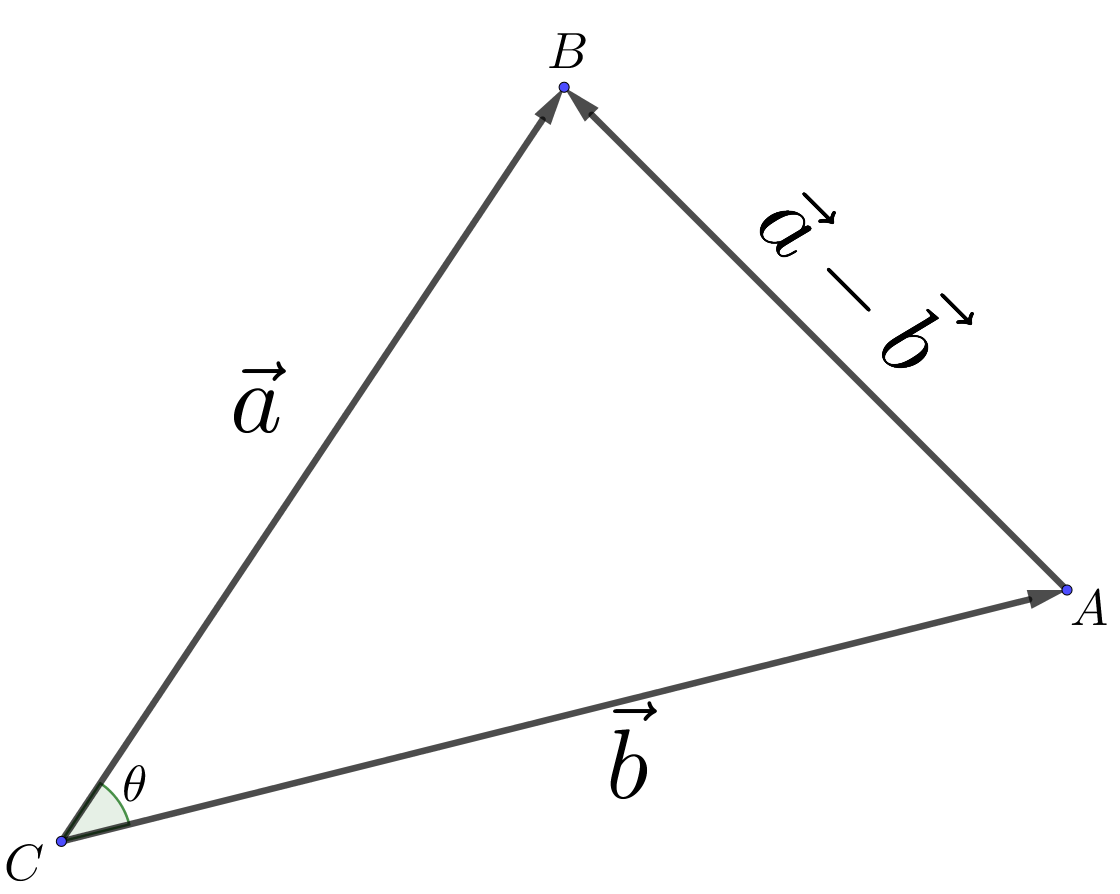
\includegraphics[width=0.45\textwidth]{angleBetweenVectors}
                    \caption{Ángulo entre Vectores}
                \end{figure}

                % ======== DEMOSTRACION ========
                \begin{SmallIndentation}[1em]
                    
                    Ve la foto, y vamos a ver que pasa:
                    \begin{MultiLineEquation*}{3}
                        \Abs{\vec a - \vec b}^2 
                            &= \Abs{\vec a }^2 + \Abs{\vec b}^2 - 2 \Abs{\vec a } \Abs{\vec b } \cos\theta
                                && \Remember{Al aplicar la Ley de Cosenos tenemos esto}                                     \\
                        \Wrap{\vec a - \vec b } \dotP \Wrap{\vec a - \vec b } 
                            &= \vec a  \dotP \vec a + \vec b \dotP \vec b - 2\Abs{\vec a}\Abs{\vec b}\cos\theta
                                && \Remember{Definición alterna de magnitud (producto punto)}                               \\
                        \vec a \dotP \Wrap{\vec a-\vec b} - \vec b \dotP \Wrap{\vec a-\vec b} 
                            &= \vec a \dotP \vec a + \vec b \dotP \vec b - 2\Abs{\vec a}\Abs{\vec b}\cos\theta        
                                && \Remember{Aplicamos la propiedad de linearidad}                                          \\
                        \vec a \dotP \vec a - 2\vec a \dotP \vec b + \vec b \dotP \vec b 
                            &= \vec a \dotP \vec a + \vec b \dotP \vec b - 2\Abs{\vec a}\Abs{\vec b}\cos\theta        
                                && \Remember{Aplicamos la propiedad de conmutativa}                                         \\
                        - 2\vec a \dotP \vec b 
                            &= - 2\Abs{\vec a}\Abs{\vec b}\cos\theta
                                && \Remember{Cancelamos términos comunes}                                                        
                    \end{MultiLineEquation*}

                    \begin{Definition}[Definición Alterna del Producto Punto con Magnitud]
                        \begin{equation}
                            \vec a \dotP \vec b = \Abs{\vec a} \Abs{\vec b} \cos\theta
                        \end{equation}
                    \end{Definition}

                \end{SmallIndentation}

                La ecuación anterior es una de las más importantes que involucran al producto punto,
                pues ahora lo relaciona con las magnitudes de los vectores y el ángulo entre ellos.
                
                \textbf{A veces es común encontrar dicha ecuación como definición de producto punto
                y la que nosotros propusimos como consecuencia, ambas formas son correctas, pero
                creemos que es más fácil definirla de forma algebráica y luego deducir la forma
                geométrica}.



                    
            % =========================================================
            % =============    VECTORES ORTOGONALES     ===============
            % =========================================================
            \clearpage
            \subsection{Definición de los Vectores Ortogonales por P. Punto}
                    
                Ahora, usando la ecuación $\vec a \dotP \vec b = \Abs{\vec a} \Abs{\vec b} \cos\theta$
                simplemente podemos despejar el coseno del ángulo y obtenemos esta linda fórmula:
                \begin{align}
                    \cos \theta &= \dfrac{\vec a \dotP \vec b}{\Abs{\vec a} \Abs{\vec b}}
                \end{align}
                
                Como el rango de $\arccos$ va de $0$ a $\pi$, usando esta fórmula siempre obtendremos
                el ángulo correcto.

                Más aún, si $\theta = 90^\circ$, entonces $\vec a \dotP \vec b = 0$.
                Esto nos motiva a definir lo siguiente, pues estos vectores recibirán un nombre especial:
    
                \begin{Definition}[Vectores ortogonales]
                    \ForceNewLine
                    Sean $\vec{a}, \vec{b} \in \Reals^3$. Decimos que $\vec{a}$ y $\vec{b}$ son 
                    \textbf{ortogonales} si y solo si $\vec{a} \cdot \vec{b} = 0$.
                \end{Definition}

                Nota que el cero vector $\vec{0}$ es ortogonal a cualquier otro vector.



            % =========================================================
            % =============     PROYECCION DE VECTORES   ==============
            % =========================================================
            \clearpage
            \subsection{Proyección de un Vector sobre Otro}
            
                Ahora consideremos la siguiente situación:

                \begin{wrapfigure}{r}{0.45\textwidth}
                    \centering
                    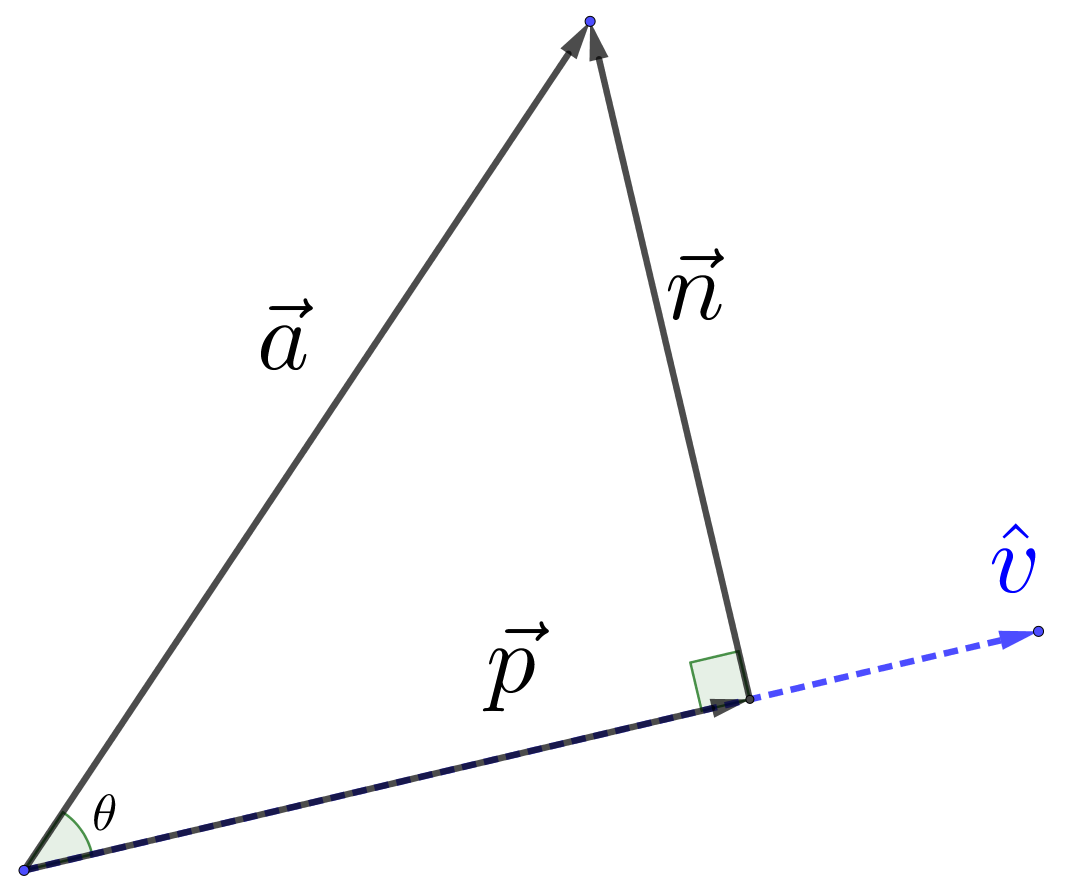
\includegraphics[width=0.42\textwidth]{vectorProyection}
                \end{wrapfigure}

                Tenemos un vector cualquiera $\vec{a}$ y un vector unitario $\hat{v}$ que forman
                entre ellos un ángulo $\theta$.
                Queremos hallar la \emph{proyección} de $\vec{a}$ sobre la línea que genera la
                dirección de $\hat{v}$.
                
                Es decir, supongamos que extendemos el vector $\hat{v}$ para que forme un \Quote{piso}.
                Luego, colocamos al vector $\vec{a}$ en el mismo origen que $\hat{v}$, esta proyección
                nos dice la sombra que generaría $\vec{a}$ sobre el piso.
                
                Llamemos a la proyección $\vec{p}$, y al vector que resulta de unir la punta de $\vec{p}$
                con la punta de $\vec{a}$ el vector $\vec{n}$ (al que llamaremos \emph{componente normal
                de $\vec{a}$ sobre $\hat{v}$}).
                
                Resulta claro que el ángulo que forma la punta de $\vec{p}$ con el inicio de $\vec{n}$
                tiene que ser de $90^\circ$ por definición.

                De esa forma, aplicamos la definición del coseno para saber la magnitud de $\vec{p}$:
                \begin{align*}
                    \Abs{ \vec p } 
                        &= \Abs{ \vec a } \cos \theta
                            && \Remember{Definición del coseno para saber $\Abs{\vec p }$}                          \\
                        &= \Abs{ \vec a } \dfrac{\vec{a} \dotP \hat{v}}{\Abs{\vec{a}} \Abs{\hat{v}}}
                            && \Remember{Sabemos que...}                                                            \\
                         &= \Abs{ \vec a } \dfrac{\vec{a} \dotP \hat{v}}{\Abs{\vec{a}}}
                            && \Remember{Recuerda que es un vector unitario}                                        \\
                        &= \cancel{\Abs{\vec a }} \dfrac{\vec a \dotP \hat v }{\cancel{\Abs{\vec a }}} 
                            && \Remember{Cancelamos cosas}                                                          \\
                        &= \vec{a} \dotP \hat{v}
                            && \Remember{¡Bingo!}
                \end{align*}
            
                Ya tenemos la magnitud de $\vec{p}$, para determinarlo completamente solo nos hace falta su
                dirección, pero es claro que tiene que ser la misma de $\hat{v}$, y como $\hat{v}$ es unitario,
                simplemente multiplicamos:
                \begin{align*}
                    \vec{p} = \Abs{\vec{p}} \hat{v} 
                        \implies
                    \vec{p} = \Wrap{\vec{a} \dotP \hat{v}} \hat{v}
                \end{align*}
                
                Finalmente, vemos de la figura que $\vec{p} + \vec{n} = \vec{a}$, entonces $\vec{n} = \vec{a} - \vec{p}$:
                \begin{align*}
                    \vec{n} = \vec{a} - \Wrap{\vec{a} \dotP \hat{v}} \hat{v}
                \end{align*}
                
                Los dos vectores anteriores son muy importantes que conviene \emph{definirlos}.



                
                % =========================================================
                % =================     DEFINICION   ======================
                % =========================================================
                \clearpage

                    \begin{Definition}[Proyección de Vectores]
                        \ForceNewLine
                        Sean $\vec{a}, \hat{v} \in \Reals^3$ con $\hat{v}$ unitario.
                        
                        Definimos a la \textbf{Proyección de $\vec{a}$ sobre $\hat{v}$} como:
                        \begin{align}
                            proy_{\hat{v}}(\vec{a}) := \Wrap{\vec{a} \dotP \hat{v}} \hat{v}
                        \end{align}
                        
                        Y a la \textbf{componente normal de $\vec{a}$ sobre $\hat{v}$} como:
                        \begin{align}
                            \vec{n} := \vec{a} - \Wrap{\vec{a} \dotP \hat{v}} \hat{v}
                        \end{align}

                    \end{Definition}
                
                    Si $\vec{v}$ no fuera unitario, simplemente lo normalizamos, además de que la fórmula
                    se ve bonita asumiendo que es unitario.

                    Si no lo fuera, tendríamos que:
                    \begin{align}
                        proy_{\vec{v}}(\vec{a}) := \dfrac{\Wrap{\vec{a} \dotP \vec{v}}\vec{v}}{\Abs{\vec{v}}^2}
                    \end{align}




            % =========================================================
            % ==============     COSENOS DIRECTORES   =================
            % =========================================================
            \clearpage
            \subsection{Cosenos Directores}
                
                Esta es una sección sencilla, se refiere a que dado un vector $\vec{a} = (a_1, a_2, a_3)$,
                lo proyectemos sobre los tres ejes $\mathbf{x}$, $\mathbf{y}$, $\mathbf{z}$ y obtengamos
                los tres ángulos.
                
                Para proyectarlo sobre el eje $\mathbf{x}$, tenemos que proyectar $\vec{a}$ sobre el vector
                unitario $\hat{i}$. Nombremos $\alpha$ al ángulo que forman, entonces:
                \begin{align}
                    \cos \alpha 
                        = \dfrac{\vec{a} \dotP \hat{i}}{\Abs{\vec{a}} \Abs{\hat{i}}}
                        = \dfrac{a_1}{\Abs{\vec{a}}}
                \end{align}
                
                Hacemos lo mismo con los otros ejes (el ángulo $\beta$ para el eje $\mathbf{y}$, $\gamma$
                para el eje $\mathbf{z}$) y obtenemos:
                \begin{align}
                    \cos \beta  &= \dfrac{a_2}{\Abs{\vec{a}}}           \\
                    \cos \gamma &= \dfrac{a_3}{\Abs{\vec{a}}}
                \end{align}
                
                De esta forma, podemos escribir al vector unitario de $\vec{a}$ como:
                \begin{equation*}
                    \hat{a} = (\cos \alpha)\hat{i} + (\cos \beta)\hat{j} + (\cos \gamma)\hat{k}
                \end{equation*}

                Se queda como ejercicio que demuestres que $\hat{a}$ es realmente unitario :p
                
        


            % =========================================================
            % ================     CAUCHY-SCHWARZ   ===================
            % =========================================================
            \clearpage
            \subsection{Desigualdad de Cauchy-Schwarz}
            
                Esta es una de las desigualdades más poderosas, tanto que es muy usada en álgebra lineal.
                
                \begin{Theorem}[Desigualdad de Cauchy-Schwarz]
                    \ForceNewLine
                    Sean $\vec{a}, \vec{b} \in \Reals^3$. Entonces:
                    \begin{align}
                        \abs{\vec{a} \dotP \vec{b}} \leq \Abs{\vec{a}} \Abs{\vec{b}} \label{CS-Inequality}
                    \end{align}
                \end{Theorem}

                Es decir, el valor absoluto del producto punto de dos vectores siempre será menor o igual al producto
                de sus magnitudes.

                % ======== DEMOSTRACION ========
                \begin{SmallIndentation}[1em]
                    \textbf{Demostración}:
                    
                    En este librito es suficiente con demostrarla para el espacio $\Reals^3$.
                    Aunque también es válida para cualquier tipo de vectores de cualquier espacio vectorial
                    con un producto interno.
                    
                    Supongamos que ningún vector es el cero vector. Si alguno lo fuera su magnitud sería cero
                    y la desigualdad de Cauchy-Schwarz se cumple trivialmente.
                    
                    Sea $\theta$ el ángulo que forman $\vec{a}$ y $\vec{b}$. De trigonometría sabemos que 
                    $-1 \leq \cos \theta \leq 1$, entonces $\abs{\cos \theta} \leq 1$.

                    Pero anteriormente deducimos que $\cos \theta = \frac{\vec{a} \cdot \vec{b}}{\Abs{\vec{a}} \Abs{\vec{b}}}$,
                    entonces $\abs{\frac{\vec{a} \cdot \vec{b}}{\Abs{\vec{a}} \Abs{\vec{b}}}} \leq 1$, lo que implica que
                    $\Abs{\vec{a} \dotP \vec{b}} \leq \Abs{\vec{a}} \Abs{\vec{b}}$.

                    Una forma alternativa de esta desigualdad es usando la definición de valor absoluto
                    (similar al coseno anteriormente):
                    \begin{equation*}
                        -\Abs{\vec{a}} \Abs{\vec{b}} 
                            \leq 
                                \vec{a} \dotP \vec{b}
                                    \leq
                                        \Abs{\vec{a}} \Abs{\vec{b}}   
                    \end{equation*}
                
                \end{SmallIndentation}



            % =========================================================
            % ==========     DESIGUALDAD DEL TRIÁNGULO   ==============
            % =========================================================
            \clearpage
            \subsection{Desigualdad del Triángulo}

                \begin{wrapfigure}{r}{0.30\textwidth}
                    \centering
                    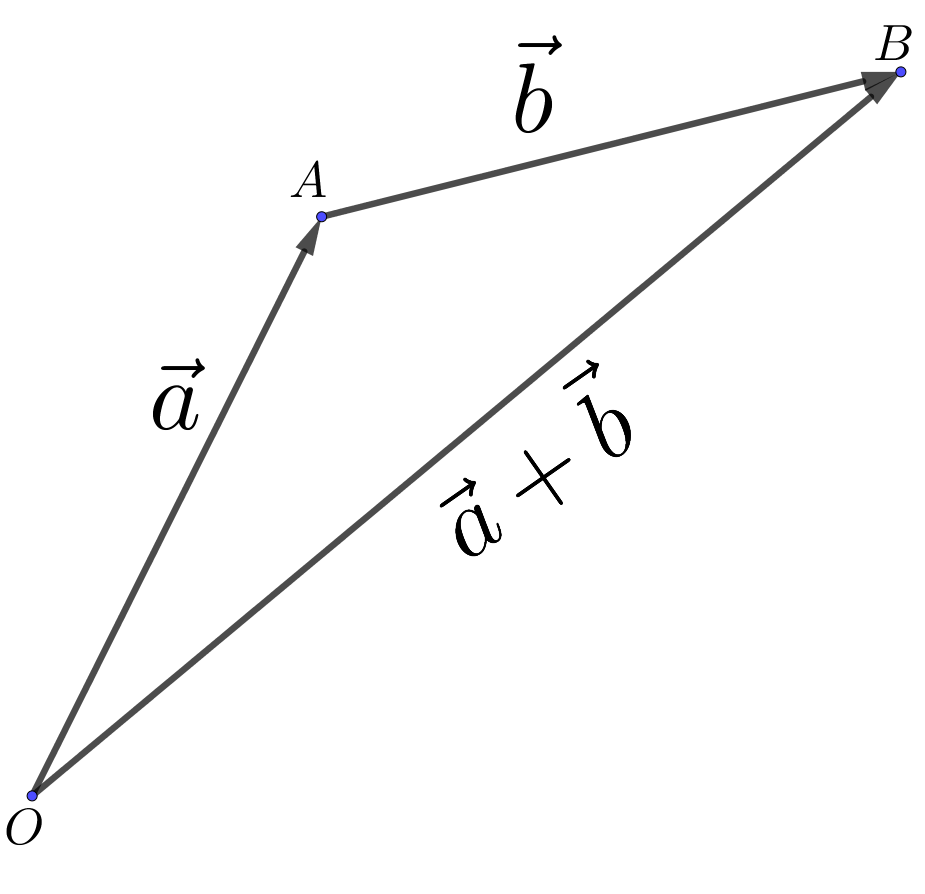
\includegraphics[width=0.25\textwidth]{triangleInequality.png}
                    \label{Con dibujitos :3}
                \end{wrapfigure}
            
                Es muy intuitiva de comprender, dice que la magnitud de la suma de dos vectores es menor o
                igual a la suma de sus magnitudes. Formalmente:
                
                \begin{Theorem}[Desigualdad del Triángulo]
                    \ForceNewLine
                    Sean $\vec{a}, \vec{b} \in \Reals^3$. Entonces:
                    \begin{align*}
                        \Abs{\vec{a}+\vec{b}} \leq \Abs{\vec{a}} + \Abs{\vec{b}}
                    \end{align*}
                \end{Theorem}
            
                Vemos que la distancia más corta entre el origen $O$ y el punto $B$ tiene que ser
                un segmento de recta, justamente $\Abs{\vec{a} + \vec{b}}$.

                Si en vez de irnos directamente a $B$ nos vamos primero a $A$ y de ahí a $B$, habremos
                recorrido una mayor distancia, que es $\Abs{\vec{a}} + \Abs{\vec{b}}$

                Pero claro, eso no es una demostración formal. Aquí viene la chida:

                % ======== DEMOSTRACION ========
                \begin{SmallIndentation}[1em]
                    \textbf{Demostración:}

                    Tratemos de usar todo lo aprendido hasta ahora, en especial el producto punto y la
                    desigualdad de Cauchy-Schwarz.

                    Comencemos del lado de $\Abs{\vec{a} + \vec{b}}$, pero elevado al cuadrado para poder
                    pasar a producto punto sin que haya raíces:
                    \begin{align*}
                        \Abs{\vec{a}+\vec{b}}^2
                            &= \Wrap{\vec{a} + \vec{b}} \dotP \Wrap{\vec{a} + \vec{b}}
                                &&\Remember{Definición de magnitud}                                     \\
                            &= \vec{a} \dotP \vec{a} 
                              + 2 \textcolor{DeepPurpleMD}{\vec{a} \dotP \vec{b}}
                              + \vec{b} \dotP \vec{b} 
                                &&\Remember{Propiedad distributiva}                                     \\
                            &\textcolor{DeepPurpleMD}{\leq} \;\; \vec{a} \dotP \vec{a}
                              + 2\textcolor{DeepPurpleMD}{\Abs{\vec{a}}\Abs{\vec{b}}} 
                              + \vec{b} \dotP \vec{b}
                                &&\textcolor{DeepPurpleMD}{\Remember{Desigualdad de Cauchy-Schwarz}}    \\
                            &= \Abs{\vec{a}}^2 + 2\Abs{\vec{a}} \Abs{\vec{b}} + \Abs{\vec{b}}^2 
                                &&\Remember{Definición de magnitud a la inversa}                        \\
                            &= \Wrap{\Abs{\vec{a}} + \Abs{\vec{b}}}^2 
                                &&\Remember{Factorizamos}
                    \end{align*}
                    
                    De esa forma obtenemos $\Abs{\vec{a}+\vec{b}}^2 \leq \Wrap{\Abs{\vec{a}} + \Abs{\vec{b}}}^2$.

                    Como todas las magnitudes son no negativas, podemos sacar raíz cuadrada a ambos lados y
                    concluir que $\Abs{\vec{a}+\vec{b}} \leq \Abs{\vec{a}} + \Abs{\vec{b}}$.

                \end{SmallIndentation}
            





        
        % =========================================================
        % =================     PRODUCTO CRUZ   ===================
        % =========================================================
        \clearpage
        \section{Producto Cruz}
        
            Es el segundo tipo de producto que existe entre los vectores.

            Este sí es un producto \Quote{genuino} de vectores, porque el resultado ahora sí es otro vector. 
            Sin embargo es un poco raro en comparación al producto punto, pues definirlo directamente de forma
            algebráica sería complicado y poco intuitivo.

            Además de que es obligatorio que trabajemos en $\Reals^3$ (porque está muy arraigado al espacio en 3D),
            pues en $\Reals^2$ no tiene sentido y en dimensiones superiores es bastante complicado generalizarlo.
            
            Dicho lo anterior, tratemos de definirlo primero de forma geométrica:
            
            % =========================================================
            % ===================     DEFINICION   ====================
            % =========================================================
            \subsection{Definición}

                \ForceNewLine
                Sean $\vec{a}, \vec{b} \in \Reals^3$. Definimos al \textbf{producto cruz} o
                \textbf{producto vectorial} de $\vec{a}$ con $\vec{b}$ como:
                \begin{align}
                    \vec{c} &= \vec{a} \times \vec{b} \label{defCross}
                \end{align}

                Donde: 

                \begin{minipage}{0.30\textwidth}
                    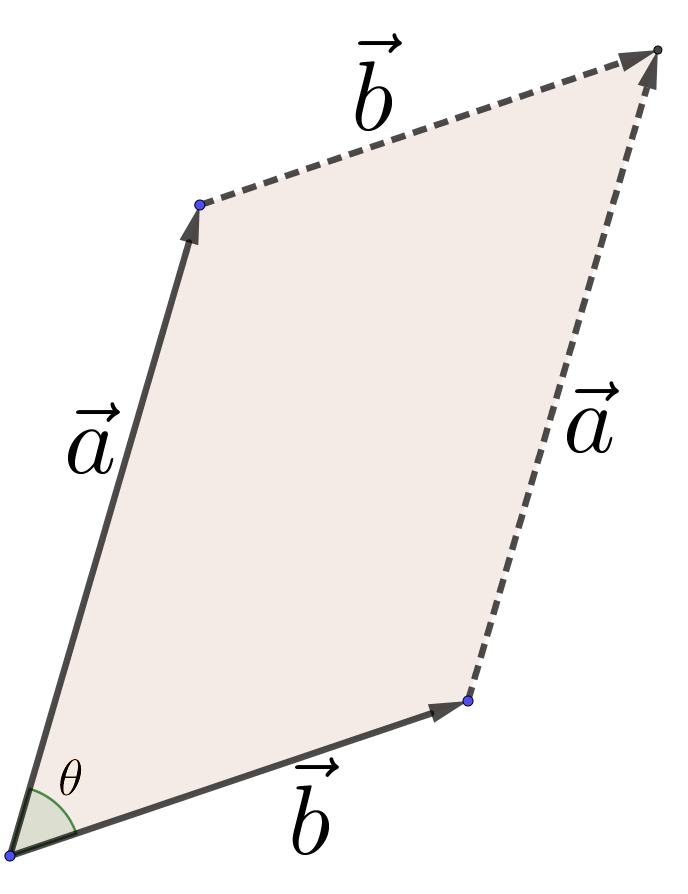
\includegraphics[width=0.60\textwidth]{parallelogram}
                \end{minipage}
                \begin{minipage}[t]{.65\textwidth}

                    $\Abs{\vec{c}}$ es el área del paralelogramo formado por los vectores $\vec{a}$ y $\vec{b}$.
                    De geometría y trigonometría sabemos que dicha área es 
                    $\Abs{\vec{c}} = \Abs{\vec{a}} \Abs{\vec{b}} \sin \theta$, donde $0 \leq \theta \leq \pi$.

                \end{minipage}

                \vspace{2em}
                
                \begin{minipage}{0.30\textwidth}
                    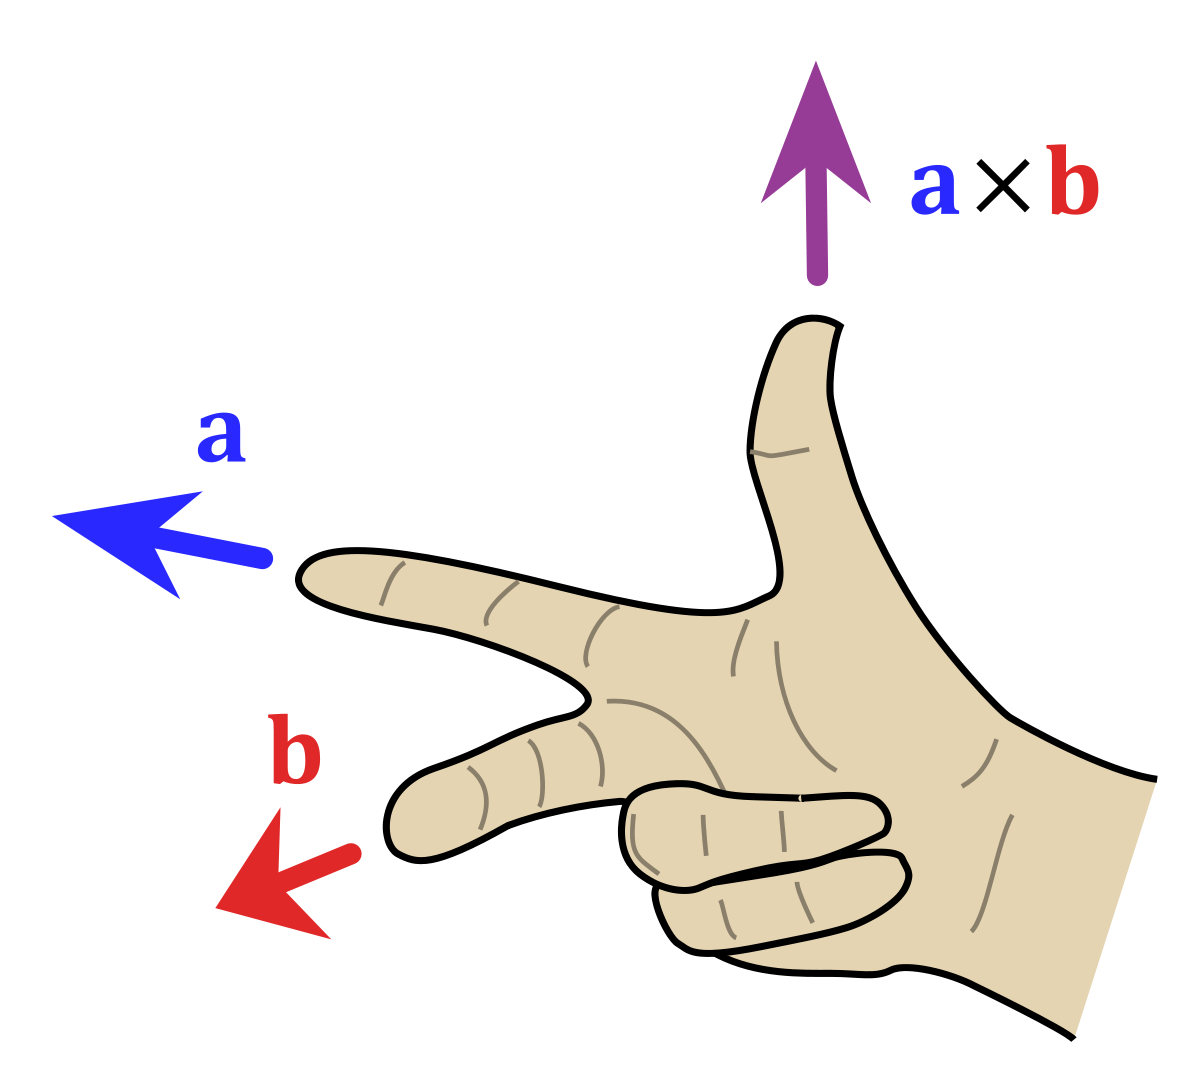
\includegraphics[width=0.80\textwidth]{rightHandRule}
                \end{minipage}
                \begin{minipage}[t]{0.65\textwidth}
                    La dirección de $\vec{c}$, es decir, $\hat{c}$, es perpendicular tanto a $\vec{a}$ como a $\vec{b}$,
                    y de forma arbitraria vamos a proponer que se siga la famosa \textbf{regla de la mano derecha},
                    porque justamente en tu mano derecha el índice lo apuntas en dirección de $\vec{a}$ y el dedo medio
                    en dirección de $\vec{b}$, tu pulgar apuntará en la dirección de $\hat{c}$.
                \end{minipage}
        

            % =========================================================
            % ===========    VECTORES UNITARIOS    ====================
            % =========================================================
            \clearpage
            \subsection{Vectores Unitarios y P. Cruz}

                Para hacer que la definición anterior sea verdaderamente útil, calculemos los
                productos cruz de los vectores unitarios canónicos $\hat{i}, \hat{j}, \hat{k}$.
                
                Si dibujamos los vectores $\hat{i}$ y $\hat{j}$, vemos que el paralelogramo que
                forman es justamente un cuadrado de área 1, pues el lado mide 1:
                \begin{figure}[H]
                    \centering
                    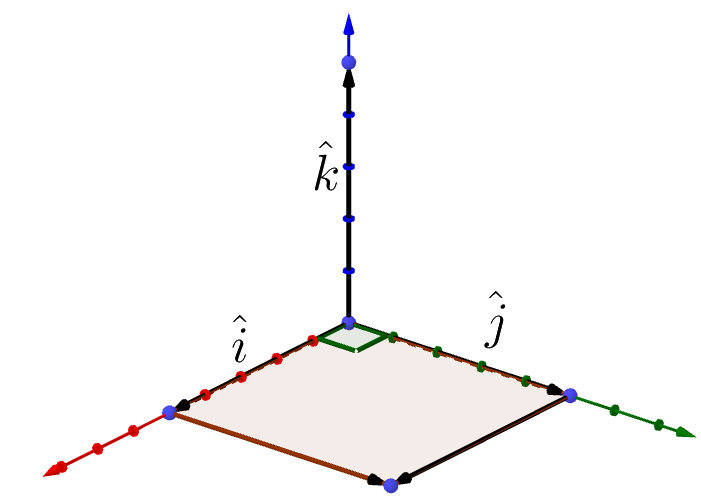
\includegraphics[width=0.60\textwidth]{unitVectors}
                \end{figure}
            
                De esta forma, $\abs{\hat{i} \times \hat{j}} = 1$. También vemos que cualquier
                dirección perpendicular a $\hat{i}$ y a $\hat{j}$ simultáneamente tiene que apuntar
                a fuerzas hacia $\pm \hat{k}$. Pero por la regla de la mano derecha, nos quedamos con
                la positiva.

                Por lo tanto: $\hat{i} \times \hat{j} = \hat{k}$. De forma similar tomando los otros
                posibles pares de vectores unitarios canónicos, obtenemos las siguientes relaciones:

                % ==================================================
                % ===========    FORMULAS UTILES    ================
                % ==================================================
                \vspace{1.5em}
                \textbf{Definiciones usando Producto Cruz}
                    \begin{align*}
                        \textcolor{Teal700MD}
                        {\hat{i} = \hat{j} \times \hat{k}}
                            \MegaSpace \MegaSpace \Space
                        \textcolor{Indigo700MD}
                        {\hat{j} = \hat{k} \times \hat{i}}
                            \MegaSpace \MegaSpace \Space
                        \textcolor{Amber900MD}
                        {\hat{k} = \hat{i} \times \hat{j}}
                    \end{align*}

                % ==================================================
                % ===========    CREANDO VECTORES CERO     =========
                % ==================================================
                \textbf{Creando Vectores Cero}
                    \begin{align*}
                        \textcolor{RedMD}
                            {\hat{0}}
                            \;
                        \textcolor{Teal700MD}
                            { = \hat{i} \times \hat{i}}
                            \;
                        \textcolor{Indigo700MD}
                            { = \hat{j} \times \hat{j}}
                            \;
                        \textcolor{Amber900MD}
                            { = \hat{k} \times \hat{k}}
                    \end{align*}

                % ==================================================
                % ===========      COSAS RARAS      ================
                % ==================================================
                \textbf{Cosas Raras}
                    \begin{align*}
                        \textcolor{Teal700MD}
                        {-\hat{i} = \hat{k} \times \hat{j}}
                            \MegaSpace \MegaSpace
                        \textcolor{Indigo700MD}
                        {-\hat{j} = \hat{i} \times \hat{k}}
                            \MegaSpace \MegaSpace
                        \textcolor{Amber900MD}
                        {-\hat{k} = \hat{j} \times \hat{i}}
                    \end{align*}
                    


            % =========================================================
            % ===========    PROPIEDADES GENERALES   ==================
            % =========================================================
            \clearpage
            \subsection{Propiedades Generales}

                Ahora veamos algunas propiedades básicas del producto cruz para poder deducir una fórmula
                en términos de las componentes de los vectores:
                
                Tenemos las siguientes propiedades, donde $\vec{a}, \vec{b}, \vec{c} \in \Reals^3$ y $k \in \Reals$:
                \begin{itemize}

                    \item
                        \textbf{Anticonmutatividad:}
                            $\vec{a} \times \vec{b} = -\vec{b} \times \vec{a}$

                            % ======== DEMOSTRACION ========
                            \begin{SmallIndentation}[1em]
                                \textbf{Demostración}:

                                \begin{SmallIndentation}[0.5em]
                                    
                                    \textbf{Magnitud:}

                                    Por definición, $\Abs{\vec{a} \times \vec{b}} = \Abs{\vec{a}} \Abs{\vec{b}} \sin \theta$.
                                    Como $\theta$ es en ángulo tanto \emph{entre $\vec{a}$ y $\vec{b}$} como 
                                    \emph{entre $\vec{b}$ y $\vec{a}$}, entonces 
                                    $\Abs{\vec{a} \times \vec{b}} = \Abs{\vec{b} \times \vec{a}}$.
                            
                                    \textbf{Sentido:}

                                    Ahora, usando regla de la mano derecha, si el dedo índice apunta en dirección
                                    de $\hat{a}$ y el medio en dirección de $\hat{b}$, el pulgar apuntará en dirección
                                    de $\vec{a} \times \vec{b}$.
                                    Por lo que si ahora el dedo índice apunta en dirección de $\hat{b}$ y el medio en
                                    dirección de $\hat{a}$, es obvio que el pulgar apuntará en dirección contraria a la
                                    que apuntaba antes.
                                
                                \end{SmallIndentation}
                        
                                Concluyendo, $\vec{a} \times \vec{b} = -\vec{b} \times \vec{a}$.
                            
                            \end{SmallIndentation}
                                
                    
                    \item \textbf{Distributiva por la Izquierda:} 
                        $\vec{a} \times \Wrap{\vec{b}+\vec{c}} = \vec{a} \times \vec{b} + \vec{a} \times \vec{c}$

                        % ======== DEMOSTRACION ========
                        \begin{SmallIndentation}[1em]
                            \textbf{Demostración}:
                            Pendiente XD
                        
                        \end{SmallIndentation}
                            
                    
                    \item \textbf{Distributiva por la Derecha:}
                        $\Wrap{\vec{a}+\vec{b}} \times \vec{c} = \vec{a} \times \vec{c} + \vec{b} \times \vec{c}$

                        % ======== DEMOSTRACION ========
                        \begin{SmallIndentation}[1em]
                            \textbf{Demostración}:
                            Pendiente XD x2
                        
                        \end{SmallIndentation}

                    \clearpage
                    
                    \item $k\Wrap{\vec{a} \times \vec{b}} = \Wrap{k \vec{a}} \times \vec{b} = \vec{a} \times \Wrap{k \vec{b}}$

                        % ======== DEMOSTRACION ========
                        \begin{SmallIndentation}[1em]
                            \textbf{Demostración}:
                            
                            Veamos que $\Wrap{k \vec{a}} \times \vec{b} = k\Wrap{\vec{a} \times \vec{b}}$.
                            Si $k = 0$, ambos lados de la ecuación son el cero vector.
                            En caso contrario, sea $\theta$ el ángulo entre $\vec{a}$ y $\vec{b}$.
                        
                            Si $k>0$, la dirección de $\Wrap{k \vec{a}} \times \vec{b}$ es la misma que la de
                            $\vec{a} \times \vec{b}$ y la de $k\Wrap{\vec{a} \times \vec{b}}$.
                            El ángulo entre $k\vec{a}$ y $\vec{b}$ también es el mismo que entre $\vec{a}$ y $\vec{b}$.

                            Entonces:
                            \begin{align*}
                                \Abs{(k\vec{a}) \times \vec{b}} 
                                    &= \Abs{k\vec{a}} \Abs{\vec{b}}  \sin \theta    && \Remember{Definición de producto cruz}   \\
                                    &= k \Abs{\vec{a}} \Abs{\vec{b}} \sin \theta    && \Remember{Propiedad de la magnitud}      \\
                                    &= k \Abs{\vec{a} \times \vec{b}}               && \Remember{Definición de producto cruz}   \\
                                    &= \Abs{k\Wrap{\vec{a} \times \vec{b}}}         && \Remember{Propiedad de la magnitud}
                            \end{align*}
                            Por lo tanto, en este caso $\Wrap{k\vec{a}} \times \vec{b} = k\Wrap{\vec{a} \times \vec{b}}$.
                            
                            Si $k < 0$, la dirección de $\Wrap{k\vec{a}} \times \vec{b}$ es igual que la de 
                            $\Wrap{-\vec{a}} \times \vec{b}$ y que la de $-\Wrap{\vec{a} \times \vec{b}}$, por ello
                            es la misma que la de $k\Wrap{\vec{a} \times \vec{b}}$.

                            Entonces el ángulo entre $k\vec{a}$ y $\vec{b}$ es el suplementario del que existe entre
                            $\vec{a}$ y $\vec{b}$, es decir, $\pi-\theta$.

                            Por lo tanto:
                            \begin{align*}
                                \Abs{(k\vec{a}) \times \vec{b}} 
                                    &= \Abs{k\vec{a}} \Abs{\vec{b}} \Sin{\pi-\theta}        &&\Remember{Definición de producto cruz}    \\
                                    &= \abs{k} \Abs{\vec{a}} \Abs{\vec{b}} \Sin{\pi-\theta} &&\Remember{Propiedad de la magnitud}       \\
                                    &= \abs{k} \Abs{\vec{a}} \Abs{\vec{b}} \sin \theta      &&\Remember{Identidad trigonométrica}       \\
                                    &= \abs{k} \Abs{\vec{a} \times \vec{b}}                 &&\Remember{Definición de producto cruz}    \\
                                    &= \Abs{k\Wrap{\vec{a} \times \vec{b}}}                 &&\Remember{Propiedad de la magnitud}
                            \end{align*}
                            Por lo tanto, también en este caso tenemos que:
                            $\Wrap{k\vec{a}} \times \vec{b} = k\Wrap{\vec{a} \times \vec{b}}$.
                            
                            Se queda como ejercicio ver que $k\Wrap{\vec{a} \times \vec{b}} = \vec{a} \times \Wrap{k \vec{b}}$
                                
                        \end{SmallIndentation}
                    
                    \item $\vec{a} \times \vec{a} = \vec{0}$

                \end{itemize}
            
                Hay que tener cuidado, porque por lo general el producto cruz \textbf{no es asociativo},
                es decir, $\vec{a} \times \Wrap{\vec{b} \times \vec{c}} \neq \Wrap{\vec{a} \times \Vector{b}} \times \vec{c}$;
                por lo tanto, la expresión $\vec{a} \times \vec{b} \times \vec{c}$ es ambigua si no se especifica en qué orden
                se deben evaluar.
                

















                

            % =========================================================
            % ===========    PROPIEDADES GENERALES   ==================
            % =========================================================
            \clearpage
            \subsection{Definición Algebráica del Producto Cruz}


                Ya con todo lo que hemos visto podemos dar la definición algebráica del producto
                cruz (la presentaremos como un teorema):

                % =========================================================
                % ===================     DEFINICION   ====================
                % =========================================================
                
                \begin{Theorem}[Definición algebráica de producto cruz]
                    Sean $\vec{a}, \vec{b} \in \Reals^3$ dados por sus coordenadas: $\vec{a}=a_1\hat{i} + a_2\hat{j} + a_3\hat{k}$ y $\vec{b}=b_1\hat{i} + b_2\hat{j} + b_3\hat{k}$. Entonces:
                    \begin{align}
                        \vec{a} \times \vec{b} &=
                        \begin{vmatrix}
                            \hat{i} & \hat{j} & \hat{k}\\
                            a_1 & a_2 & a_3\\
                            b_1 & b_2 & b_3
                        \end{vmatrix}
                        = \begin{vmatrix}
                            a_2 & a_3\\
                            b_2 & b_3
                        \end{vmatrix}\hat{i} - 
                        \begin{vmatrix}
                            a_1 & a_3\\
                            b_1 & b_3
                        \end{vmatrix}\hat{j} + 
                        \begin{vmatrix}
                            a_1 & a_2\\
                            b_1 & b_2
                        \end{vmatrix}\hat{k}\\
                        &= (a_2b_3-a_3b_2)\hat{i} + (a_3b_1-a_1b_3)\hat{j} + (a_1b_2-a_2b_1)\hat{k}
                    \end{align}
                \end{Theorem}
            
                % =========================================================
                % ==================     DEMOSTRACION   ===================
                % =========================================================
                
                \begin{SmallIndentation}
                    \textbf{Demostración:} usando todas las propiedades anteriores, tenemos que (esto se pone intenso):
                    \begin{align*}
                        \vec{a} \times \vec{b} &= \Wrap{a_1\hat{i} + a_2\hat{j} + a_3\hat{k}} \times \Wrap{b_1\hat{i} + b_2\hat{j} + b_3\hat{k}}\\
                        &= \textcolor{blue}{\Wrap{a_1\hat{i} + a_2\hat{j} + a_3\hat{k}} \times \Wrap{b_1\hat{i}}}
                        + \textcolor{red}{\Wrap{a_1\hat{i} + a_2\hat{j} + a_3\hat{k}} \times \Wrap{b_2\hat{j}}}
                        + \textcolor{brown}{\Wrap{a_1\hat{i} + a_2\hat{j} + a_3\hat{k}} \times \Wrap{b_3\hat{k}}}\\
                        &= \textcolor{blue}{\cancel{a_1b_1\hat{i}\times\hat{i}} + a_2b_1\hat{j}\times\hat{i} + a_3b_1\hat{k}\times\hat{i}}
                        + \textcolor{red}{a_1b_2\hat{i}\times\hat{j} + \cancel{a_2b_2\hat{j}\times\hat{j}} + a_3b_2\hat{k}\times\hat{j}}
                        + \textcolor{brown}{a_1b_3\hat{i}\times\hat{k} + a_2b_3\hat{j}\times\hat{k} + \cancel{a_3b_3\hat{k}\times\hat{k}}}\\
                        &= -a_2b_1\hat{k} + a_3b_1\hat{j} + a_1b_2\hat{k} - a_3b_2\hat{i} - a_1b_3\hat{j} + a_2b_3\hat{i}\\
                        &= (a_2b_3 - a_3b_2)\hat{i} - (a_1b_3 - a_3b_1)\hat{j} + (a_1b_2 - a_2b_1)\hat{k}\\
                        &= \begin{vmatrix}
                            a_2 & a_3\\
                            b_2 & b_3
                        \end{vmatrix}\hat{i} - 
                        \begin{vmatrix}
                            a_1 & a_3\\
                            b_1 & b_3
                        \end{vmatrix}\hat{j} + 
                        \begin{vmatrix}
                            a_1 & a_2\\
                            b_1 & b_2
                        \end{vmatrix}\hat{k}\\
                        &= \begin{vmatrix}
                            \hat{i} & \hat{j} & \hat{k}\\
                            a_1 & a_2 & a_3\\
                            b_1 & b_2 & b_3
                        \end{vmatrix}
                    \end{align*}
                \end{SmallIndentation}
            
                Lo ideal es simplemente memorizar la definición con el determinante, ya que las coordenadas de forma explícita no están muy sencillas. ¿Y ya viste por qué fue mejor comenzar con la definición geométrica? Haber definido al producto cruz por medio de sus coordenadas no hubiera sido nada intuitivo.
                
                Vemos también que el producto cruz nos permite calcular el ángulo entre vectores, pues:
                \begin{align}
                    \sin \theta &= \dfrac{\Abs{\vec{a} \times \vec{b}}}{\Abs{\vec{a}} \Abs{\vec{b}}} \label{angleBetweenVectorsCross}
                \end{align}
                
                Sin embargo, puede que no obtengamos el ángulo correcto, porque el rango de $\arcsen$ cuando su argumento es positivo es de $0$ a $\frac{\pi}{2}$. Por eso es un poco más conveniente usar el producto punto para esto.
                
                Aunque podemos decir que $\vec{a} \times \vec{b} = \vec{0}$ si y solo si $\vec{a}$ es paralelo a $\Vector{b}$, es decir, forman un ángulo de $0^\circ$.
            
















            \clearpage
        
            \subsection{Área de un triángulo}
            
            Si tenemos un triángulo con vértices $A$, $B$ y $C$, podemos calcular su área de una forma muy sencilla usando el producto cruz.
            
            Escogemos de forma arbitraria un vértice y calculamos los dos vectores de desplazamiento a los otros dos puntos. El área simplemente será la mitad de la magnitud del producto punto entre estos dos vectores, pues dos triángulos forman un paralelogramo.
            
            \begin{figure}[H]
                \centering
                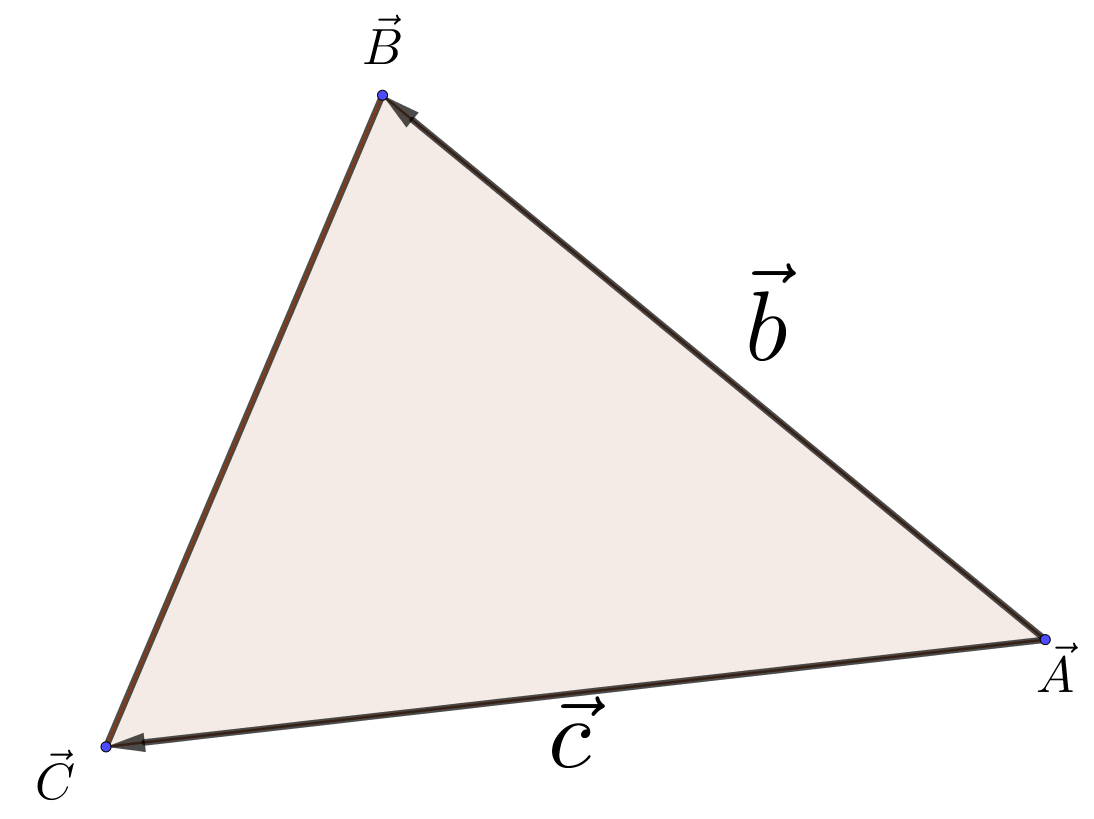
\includegraphics[scale=1.3]{triangle.png}
            \end{figure}
            
            Por ejemplo: supongamos que los vectores de posición del triángulo son $\vec{A}$, $\vec{B}$ y $\vec{C}$. Escogemos como referencia el vértice $\vec{A}$, de esta forma los vectores de desplazamiento son $\vec{b}=\vec{B}-\vec{A}$ y $\vec{c}=\vec{C}-\vec{A}$. Entonces el área será igual a $\dfrac{1}{2}\Abs{\vec{b} \times \vec{c}}$.
            
            \clearpage
            
            \subsection{Área de un paralelogramo en términos de sus diagonales}
            
            Sean $\vec{a}, \vec{b} \in \Reals^3$. Queremos hallar el área del paparelogramo que forman, pero no en términos de ellos, sino de las dos diagonales.
            
            \begin{figure}[H]
                \centering
                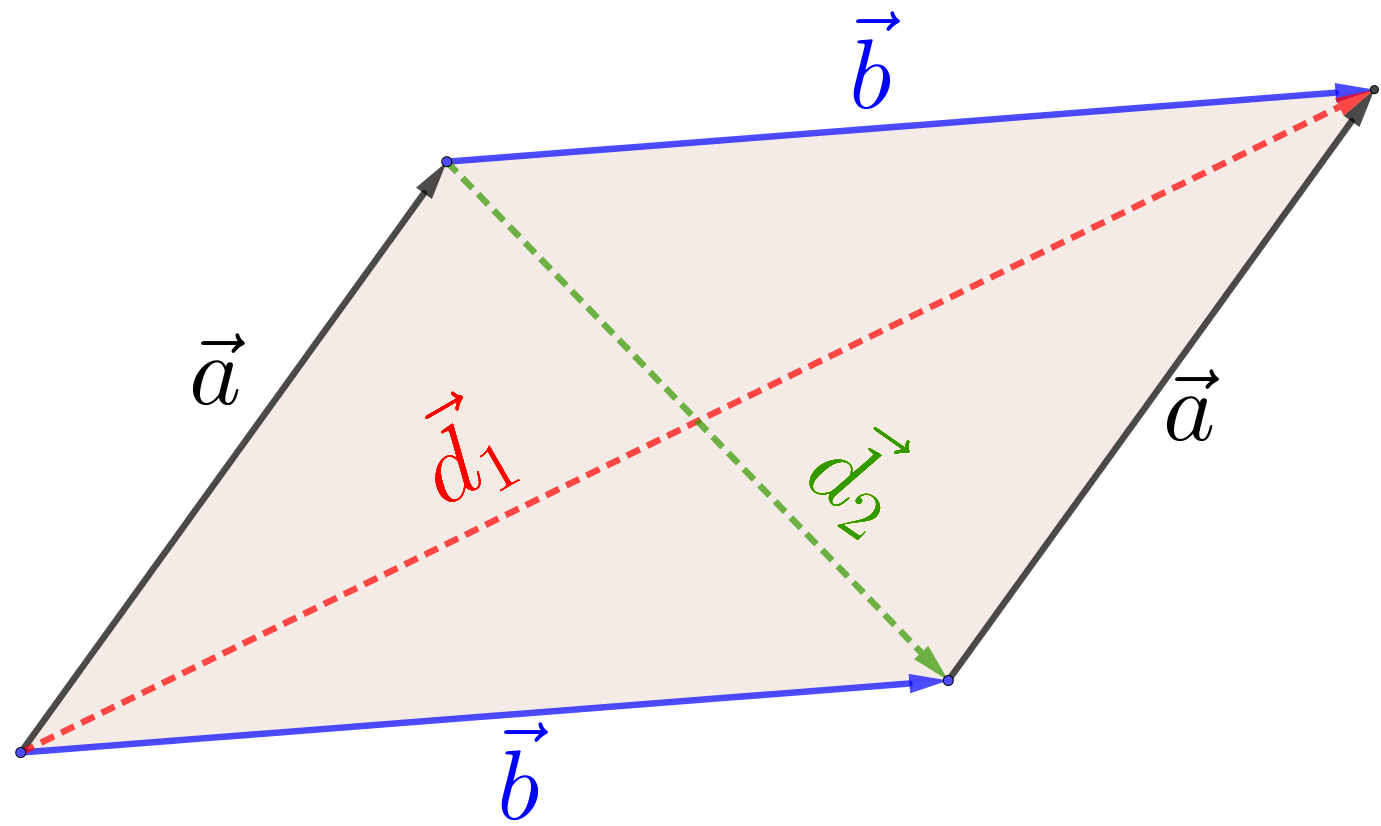
\includegraphics[scale=1.3]{parallelogram2.png}
            \end{figure}
            
            De la figura vemos que $\vec{d_1}=\vec{a}+\vec{b}$ y que $\vec{d_2}=\vec{b}-\vec{a}$, entonces hallemos $\vec{a}$ y $\vec{b}$ en términos de $\vec{d_1}$ y $\vec{d_2}$:
            \begin{align*}
                \vec{a} &= \dfrac{1}{2}\Wrap{\vec{d_1}-\vec{d_2}}\\
                \vec{b} &= \dfrac{1}{2}\Wrap{\vec{d_1}+\vec{d_2}}
            \end{align*}
            
            Por lo tanto, el área es:
            \begin{align*}
                \Abs{\vec{a} \times \vec{b}} &= \Abs{\Wrap{\dfrac{1}{2}\Wrap{\vec{d_1}-\vec{d_2}}} \times \Wrap{\dfrac{1}{2}\Wrap{\vec{d_1}+\vec{d_2}}}} = \dfrac{1}{4} \Abs{\Wrap{\vec{d_1}-\vec{d_2}} \times \Wrap{\vec{d_1}+\vec{d_2}}}\\
                &= \dfrac{1}{4}\Abs{\cancel{\vec{d_1} \times \vec{d_1}} + \vec{d_1} \times \vec{d_2} - \vec{d_2} \times \vec{d_1} - \cancel{\vec{d_2} \times \vec{d_2}}}\\
                &= \dfrac{1}{4}\Abs{\vec{d_1} \times \vec{d_2} + \vec{d_1} \times \vec{d_2}}\\
                &= \dfrac{1}{4}\Abs{2\Wrap{\vec{d_1} \times \vec{d_2}}}\\
                &= \dfrac{1}{2}\Abs{\vec{d_1} \times \vec{d_2}}
            \end{align*}
            
            \clearpage
            
            \subsection{Demostración de la ley de senos}
            A pesar de que es un teorema que es independiente del producto cruz, lo usaremos para demostrarla.
            
            \begin{figure}[H]
                \centering
                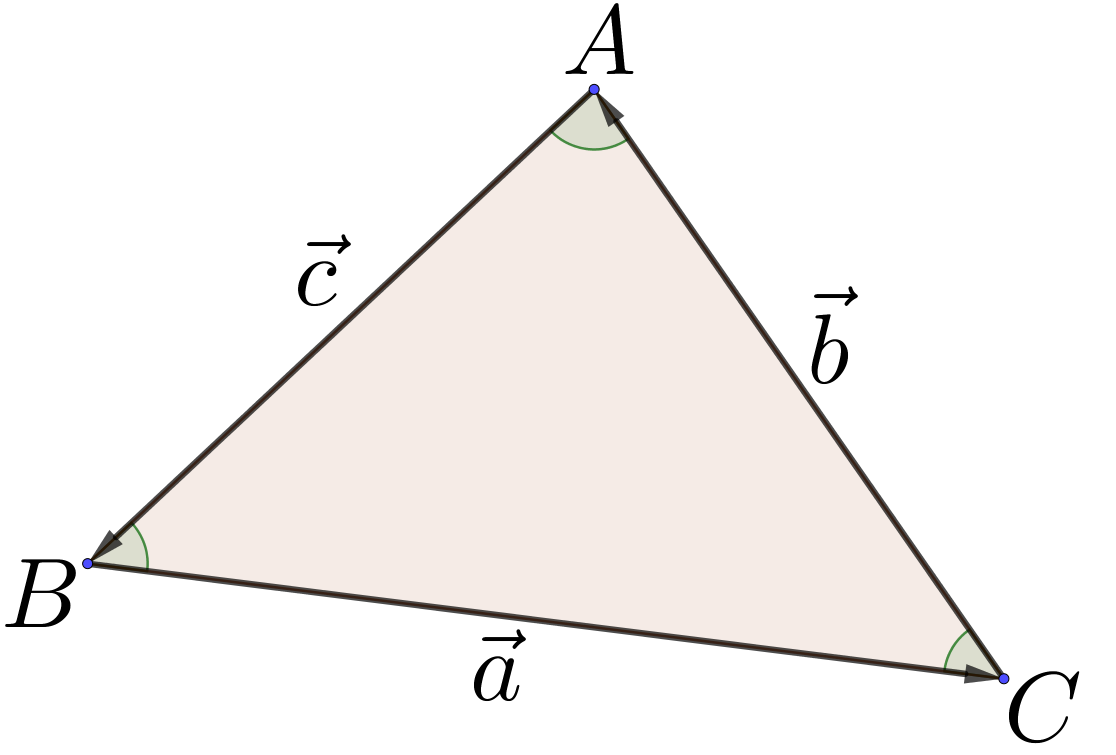
\includegraphics[scale=1.2]{sines.png}
            \end{figure}
            
            Sean $\vec{a}$, $\vec{b}$ y $\vec{c}$ los vectores de desplazamiento que representan a los lados. Es decir, $\lVec{BC}=\vec{a}$, $\lVec{CA}=\vec{b}$ y $\lVec{AB}=\vec{c}$. De la figura se ve que $\vec{a}+\vec{b}+\vec{c}=\vec{0}$, pues es cerrada.
            
            Hacemos el producto cruz con $\vec{a}$ en ambos lados:
            \begin{align}
                \Wrap{\vec{a}+\vec{b}+\vec{c}} \times \vec{a} = \vec{0} \times \vec{a} \implies \vec{b} \times \vec{a} + \vec{c} \times \vec{a} = \vec{0} \implies \vec{a} \times \vec{b} = \vec{c} \times \vec{a}
            \end{align}
            
            Ahora hacemos el producto cruz con $\vec{b}$ en ambos lados:
            \begin{align}
                \Wrap{\vec{a}+\vec{b}+\vec{c}} \times \vec{b} = \vec{0} \times \vec{b} \implies \vec{a} \times \vec{b} + \vec{c} \times \vec{b} = \vec{0} \implies \vec{a} \times \vec{b} = \vec{b} \times \vec{c}
            \end{align}
            
            Combinamos las dos ecuaciones anteriores y obtenemos que $\vec{a} \times \vec{b} = \vec{b} \times \vec{c} = \vec{c} \times \vec{a}$. Tomamos magnitud y obtenemos:
            \begin{align}
                \Abs{\vec{a}} \Abs{\vec{b}} \sin C = \Abs{\vec{b}} \Abs{\vec{c}} \sin A = \Abs{\vec{c}} \Abs{\vec{a}} \sin B
            \end{align}
            
            Reacomodamos y terminamos:
            \begin{align}
                \dfrac{\Abs{\vec{a}}}{\sin A} = \dfrac{\Abs{\vec{b}}}{\sin B} = \dfrac{\Abs{\vec{c}}}{\sin C} \label{sinesLaw}
            \end{align}
            
        % =========================================================
        % =================     PRODUCTO TRIPLE   =================
        % =========================================================
        \clearpage
        \section{Producto triple}
        
            Este no es un nuevo producto, sino más bien una combinación de los dos anteriores.
            
            \begin{Definition}[Producto triple escalar]
                Sean $\vec{a}, \vec{b}, \vec{c} \in \Reals^3$. Definimos al \textbf{producto triple escalar} como $\vec{a} \dotP \Wrap{\vec{b} \times \vec{c}}$. Nota que de nuevo el resultado es un escalar y no un vector. También se suele usar la notación $\Brackets{\vec{a}, \vec{b}, \vec{c}} = \vec{a} \dotP \Wrap{\vec{b} \times \vec{c}}$.
            \end{Definition}
        
            Tenemos la siguiente propiedad:
            
            \begin{Theorem}[Permutación circular]
                $\vec{a} \dotP \Wrap{\vec{b} \times \vec{c}} = \vec{b} \dotP \Wrap{\vec{c} \times \vec{a}} = \vec{c} \dotP \Wrap{\vec{a} \times \vec{b}}$
            \end{Theorem}
        
            \begin{SmallIndentation}[1em]
                \textbf{Demostración:} vemos que los vectores $\vec{a}+\vec{b}$ y $\Wrap{\vec{a}+\vec{b}} \times \vec{c}$ son perpendiculares por definición. Es decir, forman un ángulo de $90^\circ$. Por lo tanto:
                \begin{align*}
                    \Wrap{\vec{a}+\vec{b}} \dotP \Wrap{\Wrap{\vec{a}+\vec{b}} \times \vec{c}} &= 0 &&\mbox{Los vectores son ortogonales}\\
                    \Wrap{\vec{a}+\vec{b}} \dotP \Wrap{\vec{a} \times \vec{c} + \vec{b} \times \vec{c}} &= 0 &&\mbox{Propiedad distributiva}\\
                    \cancel{\vec{a} \dotP \Wrap{\vec{a} \times \vec{c}}} + \vec{a} \dotP \Wrap{\vec{b} \times \vec{c}} + \vec{b} \dotP \Wrap{\vec{a} \times \vec{c}} + \cancel{\vec{b} \dotP \Wrap{\vec{b} \times \vec{c}}} &= 0 &&\mbox{Propiedad distributiva}\\
                    \vec{a} \dotP \Wrap{\vec{b} \times \vec{c}} &= -\vec{b} \dotP \Wrap{\vec{a} \times \vec{c}} &&\mbox{Reacomodamos}\\
                    \vec{a} \dotP \Wrap{\vec{b} \times \vec{c}} &= \vec{b} \dotP \Wrap{\vec{c} \times \vec{a}} &&\mbox{Anticonmutatividad}
                \end{align*}
                La segunda parte de la igualdad se sigue inmediatamente, haciendo que $\vec{a} \to \vec{b}$, $\vec{b} \to \vec{c}$ y $\vec{c} \to \vec{a}$, por eso recibe el nombre de permutación circular, pues las variables se van permutando cíclicamente.
            \end{SmallIndentation}
        
            \clearpage
        
            \subsection{Volumen de un paralelepípedo}
        
            Supongamos que queremos hallar el volumen del paralelepípedo formado por los vectores $\vec{a}, \vec{b}$ y $\vec{c}$:
        
            \begin{figure}[H]
                \centering
                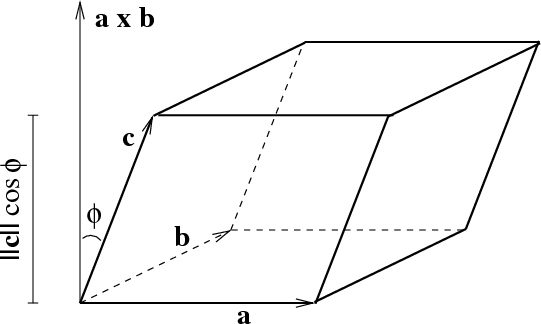
\includegraphics[scale=0.8]{parallelepiped.png}
            \end{figure}
        
            Recordemos que el volumen está dado por $V=\Wrap{\text{área de la base}}\Wrap{\text{altura}}$.
            
            Vemos que el área de la base es simplemente el área del paralelogramo formado por $\vec{a}$ y $\vec{b}$, es decir, $\Abs{\vec{a} \times \vec{b}}$.
            
            Sea $\phi$ el ángulo que forma el vector $\vec{a} \times \vec{b}$ con $\vec{c}$. Entonces, usando la definición de coseno vemos que la altura está dada por $\Abs{\vec{c}} \abs{\cos \phi}$. Usamos el valor absoluto en el coseno porque $\phi$ puede ser mayor a $90^\circ$, causando que $\cos \phi < 0$.
            
            De esa forma, el volumen es $V=\Abs{\vec{a} \times \vec{b}} \Abs{\vec{c}} \abs{\cos \phi}=\abs{\Abs{\vec{a} \times \vec{b}} \Abs{\vec{c}} \cos \phi}=\abs{\vec{c} \dotP \Wrap{\vec{a} \times \vec{b}}}$, que es justamente el valor absoluto del producto triple de los vectores que definen al paralelepípedo.
            
            ¿Qué significado tendrá el hecho de que $\vec{a} \dotP \Wrap{\vec{b} \times \vec{c}}=0$? Quiere decir que el paralelepípedo no tiene volumen, es decir, que los tres vectores \textbf{están en el mismo plano}. Veremos más adelante las propiedades del plano.
            
            La expresión \emph{producto triple} puede hacer referencia a otras combinaciones donde estén involucrados tres vectores y sus productos, como $\vec{a} \times \Wrap{\vec{b} \times \vec{c}}$, $\Wrap{\vec{a} \dotP \vec{b}}\vec{c}$, etc.
            
            Antes de terminar con esta parte, veamos un último teorema:
            
            \begin{Theorem}
                Sean $\vec{a}=a_1\hat{i}+a_2\hat{j}+a_3\hat{k}$, $\vec{b}=b_1\hat{i}+b_2\hat{j}+b_3\hat{k}$ y $\vec{c}=c_1\hat{i}+c_2\hat{j}+c_3\hat{k}$. Entonces:
                \begin{align}
                    \vec{a} \dotP \Wrap{\vec{b} \times \vec{c}} &= \begin{vmatrix}
                        a_1 & a_2 & a_3\\
                        b_1 & b_2 & b_3\\
                        c_1 & c_2 & c_3
                    \end{vmatrix} \label{tripleProduct}
                \end{align}
                Esto nos facilita mucho el cálculo del producto triple escalar, pues se reduce a que calculemos un determinante de dimensión 3, el cual es muy sencillo.
            \end{Theorem}
            
            \begin{SmallIndentation}[1em]
                \textbf{Idea de la demostración:} simplemente calcula ambos lados de la ecuación y comprueba que sean iguales. Es fácil pero tedioso.
            \end{SmallIndentation}
        
        % =========================================================
        % =================     IDENTIDADES   =====================
        % =========================================================
        
        \section{Identidades de productos}
        Existen bastantes identidades que involucran a los productos de vectores. Aquí te muestro algunas e ideas para sus demostraciones, con el fin de que seas capaz de desarrollar las tuyas propias.
        
        \begin{enumerate}\setlength\itemsep{0em}
            \item $\Abs{\vec{a} \times \vec{b}}^2 + \Wrap{\vec{a} \dotP \vec{b}}^2 = \Abs{\vec{a}}^2 \Abs{\vec{b}}^2$
            
            \begin{SmallIndentation}[1em]
                \textbf{Demostración:} Usamos las definiciones geométricas del producto punto y cruz:
                \begin{align*}
                    \Abs{\vec{a} \times \vec{b}}^2 + \Wrap{\vec{a} \dotP \vec{b}}^2 &= \Wrap{\Abs{\vec{a}} \Abs{\vec{b}} \sin \theta}^2 + \Wrap{\Abs{\vec{a}} \Abs{\vec{b}} \cos \theta}^2 &&\Remember{Definición geométrica} \\
                    &= \Abs{\vec{a}}^2 \Abs{\vec{b}}^2 \Wrap{\sin^2 \theta + \cos^2 \theta} &&\Remember{Factorizamos} \\
                    &= \Abs{\vec{a}}^2 \Abs{\vec{b}}^2 &&\Remember{Identidad trigonométrica}
                \end{align*}
            \end{SmallIndentation}
        
        
            \item $\abs{\Abs{\vec{a}} - \Abs{\vec{b}}} \leq \Abs{\vec{a} - \vec{b}}$
            
            \begin{SmallIndentation}[1em]
                \textbf{Demostración:} A esta desigualdad se le conoce como la \emph{desigualdad de triángulo en reversa}. Apliquemos la desigualdad del triángulo a los vectores $\vec{a}$ y $\vec{b}-\vec{a}$:
                \begin{align*}
                    &\Abs{\vec{a} + \Wrap{\vec{b}-\vec{a}}} \leq \Abs{\vec{a}} + \Abs{\vec{b}-\vec{a}} \implies \Abs{\vec{b}} \leq \Abs{\vec{a}} + \Abs{\vec{b}-\vec{a}} \implies \Abs{\vec{b}} - \Abs{\vec{a}} \leq \Abs{\vec{b}-\vec{a}} \\
                    &\implies -\Abs{\vec{b}-\vec{a}} \leq \Abs{\vec{a}} - \Abs{\vec{b}}
                \end{align*}
                
                Ahora a los vectores $\vec{b}$ y $\vec{a}-\vec{b}$:
                \begin{align*}
                    &\Abs{\vec{b} + \Wrap{\vec{a}-\vec{b}}} \leq \Abs{\vec{b}} + \Abs{\vec{a}-\vec{b}} \implies \Abs{\vec{a}} \leq \Abs{\vec{b}} + \Abs{\vec{a}-\vec{b}} \implies \Abs{\vec{a}} - \Abs{\vec{b}} \leq \Abs{\vec{a}-\vec{b}}
                \end{align*}
                
                Pero $\Abs{\vec{b}-\vec{a}} = \Abs{\vec{a}-\vec{b}}$, entonces podemos combinar las dos desigualdades anteriores como $-\Abs{\vec{a}-\vec{b}} \leq \Abs{\vec{a}} - \Abs{\vec{b}} \leq \Abs{\vec{a}-\vec{b}}$, y por definición de valor absoluto en los reales, la conclusión se sigue.
                
            \end{SmallIndentation}
            
            
            \item $\vec{a} \times \Wrap{\vec{b} \times \vec{c}} = \Wrap{\vec{a} \dotP \vec{c}}\vec{b} - \Wrap{\vec{a} \dotP \vec{b}}\vec{c}$
            
            \begin{SmallIndentation}[1em]
                \textbf{Demostración:} 
            \end{SmallIndentation}
            
            
            \item $\Wrap{\vec{a} \times \vec{b}} \times \Wrap{\vec{a} \times \vec{c}} = \Wrap{\vec{a} \dotP \Wrap{\vec{b} \times \vec{c}}}\vec{a}$
            
            
            \item $\Wrap{\vec{a} \times \vec{b}} \dotP \Wrap{\vec{c} \times \vec{d}} = \Wrap{\vec{a} \dotP \vec{c}} \Wrap{\vec{b} \dotP \vec{d}} - \Wrap{\vec{a} \dotP \vec{d}} \Wrap{\vec{b} \dotP \vec{c}}$
            
            
            \item $\Wrap{\vec{a} \times \vec{b}} \dotP \Wrap{\vec{c} \times \vec{d}} + \Wrap{\vec{b} \times \vec{c}} \dotP \Wrap{\vec{a} \times \vec{d}} + \Wrap{\vec{c} \times \vec{a}} \dotP \Wrap{\vec{b} \times \vec{d}} = 0$
            
            
            \item $\vec{a} \times \Wrap{\vec{b} \times \vec{c}} + \vec{b} \times \Wrap{\vec{c} \times \vec{a}} + \vec{c} \times \Wrap{\vec{a} \times \vec{b}} = \vec{0}$
        \end{enumerate}



    
    
    % ===============================================================================
    % ==============            APLICACIONES A LA GEOMETRIA         =================
    % ===============================================================================        
            
            
    \chapter{Aplicaciones a la geometría}
    
        % =========================================================
        % ====================     PLANOS   =======================
        % =========================================================
        
        \section{Ecuación del plano}
        
        El plano es un objeto bidimensional que contiene infinitos puntos y rectas. Usualmente se les denota con la letra griega $\Pi$. Para definirlo, podemos contar con la siguiente información: \begin{itemize}\setlength\itemsep{0em}
            \item Un punto por el que pasa y un vector normal a toda su superficie.
            \item Tres puntos no colineales (que no estén en la misma recta) por los que pasa.
            \item Un punto por el que pasa y dos vectores paralelos al plano.
        \end{itemize}
    
        Aunque existen muchas más combinaciones que nos pueden determinar de forma única un plano.
    
            % =========================================================
            % =============     PUNTO Y VECTOR NORMAL   ===============
            % =========================================================
    
            \clearpage
    
            \subsection{Punto y vector normal}
            
            Supongamos que el plano pasa por el punto $P$ y el vector normal a su superficie es $\vec{n}$. Queremos hallar un vector $\vec{r}$ tal que su flecha dibuje todo el plano.
            
            \begin{figure}[H]
                \centering
                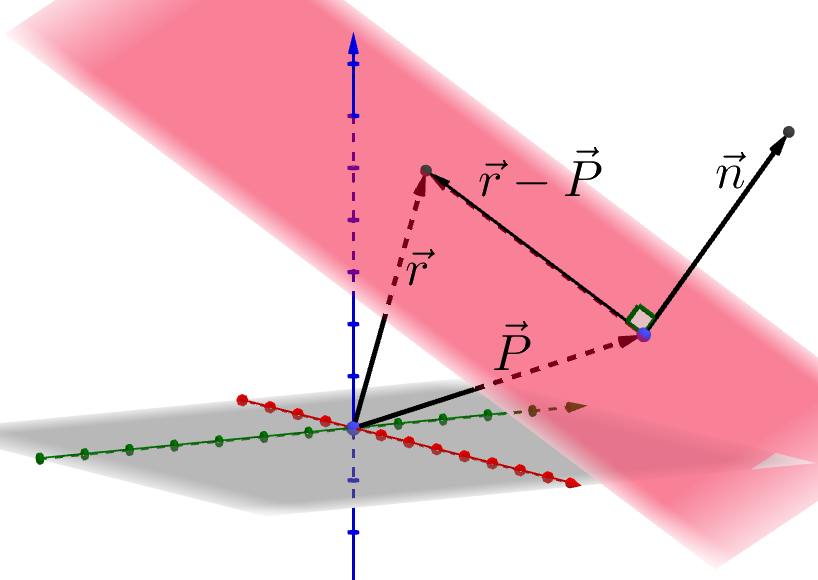
\includegraphics[scale=0.65]{plane.png}
            \end{figure}
            
            De la figura vemos que $\vec{r} - \vec{P}$ siempre está contenido en el plano, y por ser así, será perpendicular a $\vec{n}$, por lo que:
            \begin{align}
                \vec{n} \dotP \Wrap{\vec{r} - \vec{P}} &= 0 \label{planeEquationGeneral}
            \end{align}
            
            Como $\vec{r}$ se está moviendo, usemos las tres variables genéricas para representar sus coordenadas. De esa forma, supongamos que $\vec{r}=(x,y,z)$, $\vec{n}=(a,b,c)$ y $\vec{P}=(x_0, y_0, z_0)$. Entonces podemos reescribir la ecuación:
            \begin{align}
                &(a,b,c) \dotP \Wrap{x-x_0, y-y_0, z-z_0} = 0 \nonumber \\
                &\implies a(x-x_0) + b(y-y_0) + c(z-z_0) = 0 \\
                &\implies ax+by+cz = d \label{planeEquation1}
            \end{align}
            
            Donde $d=ax_0 + by_0 + cz_0$. Como puedes ver, la ecuación del plano es muy sencilla en forma cartesiana, y podemos identificar rápidamente al vector normal con tan solo fijarnos en los coeficientes. Además ten en cuenta un mismo plano puede tener más de una ecuación que lo represente (infinitas de hecho), pues cualquier múltiplo escalar del vector normal es válido.
            
            % =========================================================
            % =================     TRES PUNTOS   =====================
            % =========================================================
            
            \subsection{Tres puntos}
            
            De forma similar a como calculábamos el área de un triángulo, vamos a escoger uno de los tres puntos y hallar los vectores de desplazamiento de él hacia los otros dos:
            
            \begin{figure}[H]
                \centering
                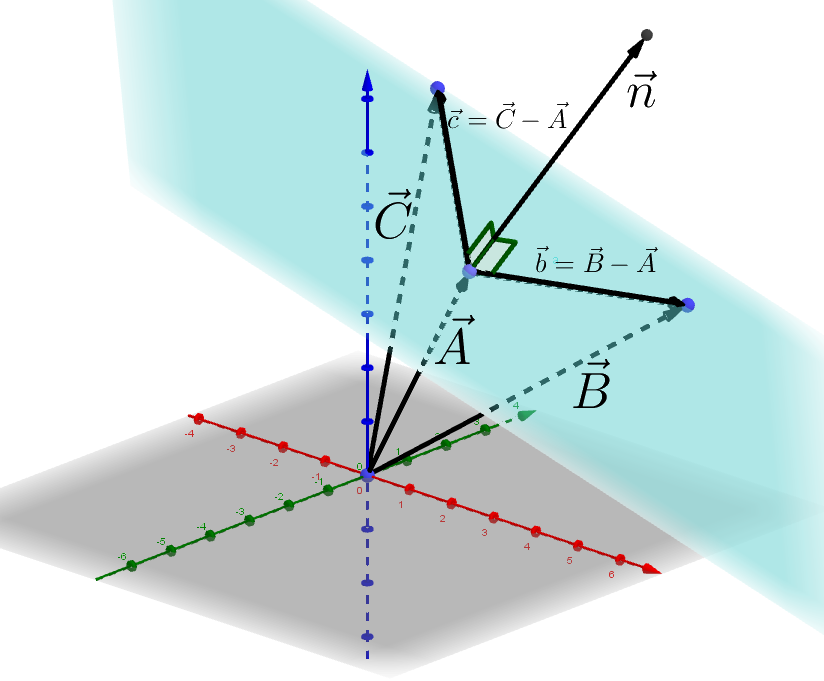
\includegraphics[scale=0.65]{plane2.png}
            \end{figure}
        
            Por ejemplo, escojamos el punto $\vec{A}$ y a partir de ahí calculemos los vectores de desplazamiento $\vec{b}=\vec{B}-\vec{A}$ y $\vec{c}=\vec{C}-\vec{A}$. Vemos que tanto $\vec{b}$ como $\vec{c}$ están contenidos totalmente en el plano, lo que nos falta es hallar el vector normal, que debe ser perpendicular a ellos dos. Por definición del producto cruz, ese vector es simplemente $\vec{n}=\vec{b} \times \vec{c}$. Finalmente, escogemos cualquiera de los tres puntos y la ecuación del plano será:
            \begin{align}
                &\vec{n} \dotP \Wrap{\vec{r} - \vec{A}} = 0 \nonumber \\
                &\implies \Wrap{\vec{b} \times \vec{c}} \dotP \Wrap{\vec{r} - \vec{A}} = 0 \label{planeEquation2}
            \end{align}
            
            La forma difícil de calcular la ecuación del plano dados tres puntos, es sustituir cada uno en la ecuación general $ax+by+cz=d$ y formar un sistema de ecuaciones para hallar $a,b,c,d$. Sin embargo, es más tardado y al hacerlo así no entendemos realmente la geometría del problema.
            
            % =========================================================
            % ========     PUNTO Y DOS VECTORES PARALELOS   ===========
            % =========================================================
            
            \subsection{Punto y dos vectores paralelos}
            
            Similar a la situación anterior, solo que ahora nos dan un punto por el que pasa ($\vec{A}$) y los dos vectores paralelos, que ahora llamaremos $\lVec{e_1}$ y $\lVec{e_2}$. Veremos que podemos escribir la ecuación del plano de otra manera:
            
            \begin{figure}[H]
                \centering
                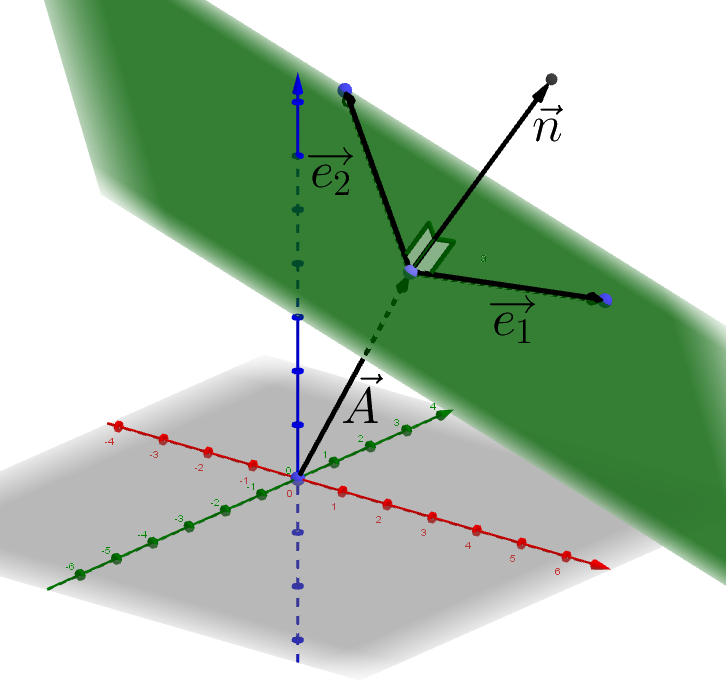
\includegraphics[scale=0.65]{plane3.png}
            \end{figure}
        
            Como el plano tiene dos dimensiones, intuitivamente podemos decir que tenemos dos \Quote{grados de libertad} de movimiento, es decir, que podemos movernos lo que queramos en la dirección de $\lVec{e_1}$ y lo que queramos en la dirección de $\lVec{e_2}$. El efecto de \Quote{movernos} no es más que multiplicar a esos vectores por un escalar. Lo que significa que cualquier punto en el plano puede ser expresado como:
            \begin{align}
                \vec{r} &= \vec{A} + s\lVec{e_1} + t\lVec{e_2} \label{planeEquation3}
            \end{align}
            
            Donde $s, t \in \Reals$, es decir, abarcan todos los números reales para \Quote{barrer} todo el plano. Le sumamos el vector $\vec{A}$ para forzar que el plano pase por ahí. Esta forma de escribir la ecuación del plano se conoce como \emph{ecuación paramétrica}, que estudiaremos más adelante.
            
            \textbf{Nota:} es muy importante que $\lVec{e_1}$ y $\lVec{e_2}$ sean linealmente independientes para poder definir un plano. ¿Qué pasaría si fueran linealmente dependientes? Pista: uno sería múltiplo escalar del otro, así que...
            
        % =========================================================
        % ====================     RECTAS   =======================
        % =========================================================
        
        \clearpage
            
        \section{Ecuación de la recta}
        
        Una recta es el conjunto de puntos que se mueven en una dirección determinada, y de forma indefinida en sus ambos extremos. Existen dos formas principales de definirlas: \begin{itemize}\setlength\itemsep{0em}
            \item Mediante un punto por el que pasa y un vector paralelo a ella.
            \item Mediante dos puntos por los que pasa.
        \end{itemize}
    
            % =========================================================
            % ============     PUNTO Y VECTOR PARALELO   ==============
            % =========================================================
            
            \clearpage
    
            \subsection{Punto y vector paralelo}
            
            Supongamos que la recta pasa por el punto $P$ y un vector paralelo a ella es $\vec{v}$. Vemos que la tarea de $\vec{v}$ es básicamente darle la dirección a la recta:
            
            \begin{figure}[H]
                \centering
                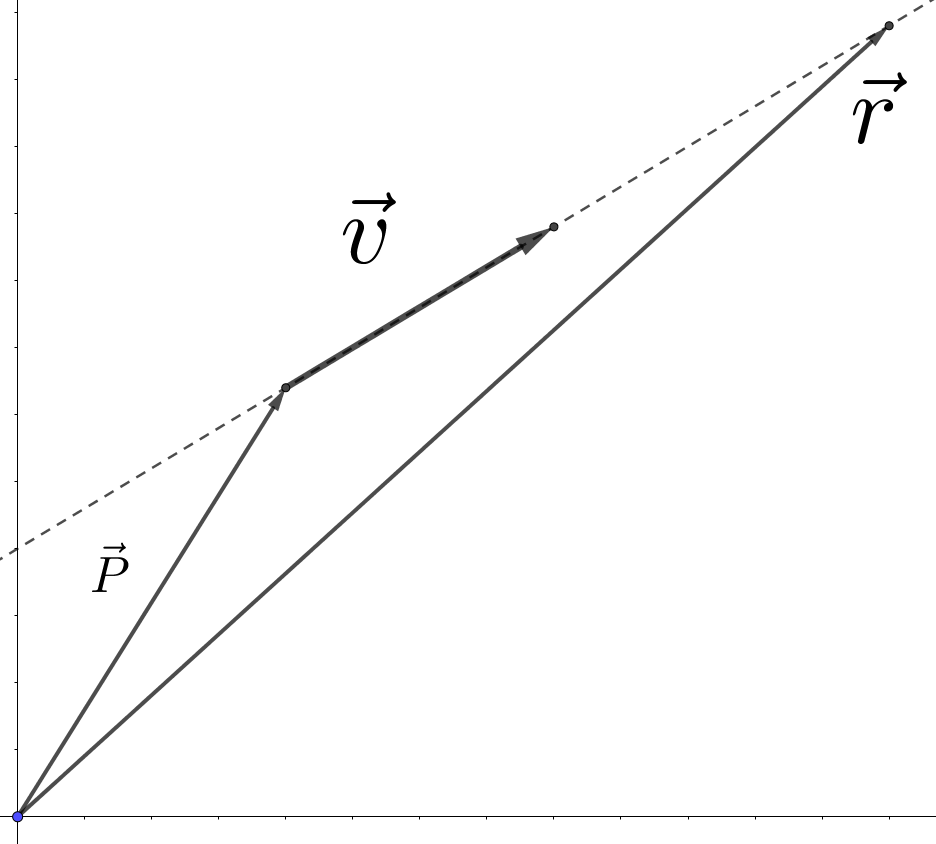
\includegraphics[scale=1.2]{line.png}
            \end{figure}
        
            Sea $\vec{r}$ el vector de posición de cada uno de los puntos de la línea, es decir, su flecha va a barrer a toda la línea. En este caso solo podemos movernos en la dirección de $\vec{v}$, por lo que cualquier múltiplo escalar de $\vec{v}$ estará sobre la línea, sumándole el punto $\vec{P}$. Entonces:
            \begin{align}
                \vec{r} &= \vec{P} + t\vec{v} \label{lineEquationGeneral}
            \end{align}
            
            Donde $t \in \Reals$. La ecuación anterior es conocida como la \emph{ecuación paramétrica de la recta}, de forma similar a la del plano. Si $\vec{r}=(x,y,z)$, $\vec{v}=(a,b,c)$ y $\vec{P}=(x_0,y_0,z_0)$, entonces podemos reescribirla como:
            \begin{align*}
                (x, y, z) &= (x_0 + ta, y_0 + tb, z_0 + tc)
            \end{align*}
            
            Comparamos componente a componente y despejamos $t$ en cada caso:
            \begin{align*}
                x &= x_0 + ta &\implies t = \dfrac{x - x_0}{a} \\
                y &= y_0 + tb &\implies t = \dfrac{y - y_0}{b} \\
                z &= z_0 + tc &\implies t = \dfrac{z - z_0}{c}
            \end{align*}
            
            Igualamos y obtenemos la forma cartesiana de la ecuación de la recta:
            \begin{align}
                \dfrac{x - x_0}{a} = \dfrac{y - y_0}{b} = \dfrac{z - z_0}{c} \label{lineEquation1}
            \end{align}
            
            Nota que una misma línea puede tener varias ecuaciones, pues cualquier múltiplo escalar de $\vec{v}$ funciona. Además, para usar la forma cartesiana requerimos que $a,b,c\neq 0$, mientras que en la forma paramétrica no hay restricción.
            
            % =========================================================
            % ==================     DOS PUNTOS   =====================
            % =========================================================
            
            \subsection{Dos puntos}
            
            Ahora supongamos que nos dan dos puntos $\vec{A}$ y $\vec{B}$, y queremos hallar la ecuación de la recta que pasa por ellos:
            
            \begin{figure}[H]
                \centering
                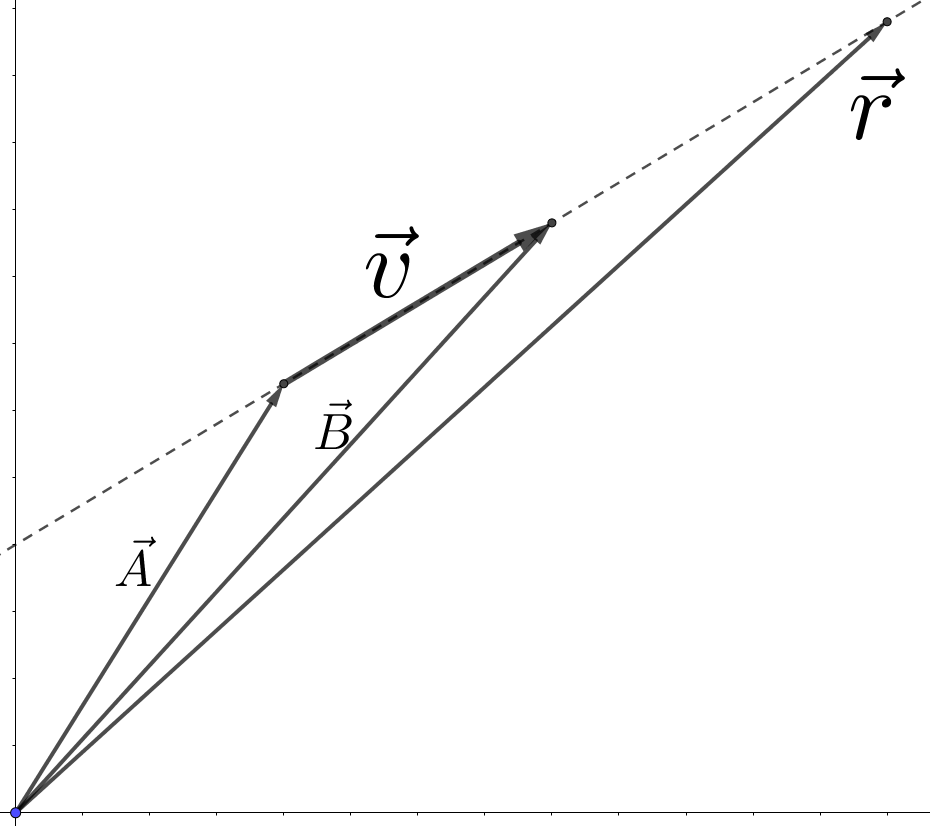
\includegraphics[scale=1.2]{line2.png}
            \end{figure}
        
            De la figura vemos que $\vec{A}+\vec{v}=\vec{B}$, entonces el vector paralelo es simplemente $\vec{v}=\vec{B}-\vec{A}$. Por lo tanto, la ecuación de la recta paramétrica queda como:
            \begin{align}
                \vec{r} &= \vec{A} + t\Wrap{\vec{B}-\vec{A}} = (1-t)\vec{A}+t\vec{B} \label{lineEquation2}
            \end{align}
            
            Nota que también podemos usar el punto $\vec{B}$ como punto inicial.
            
            Ahora, si $\vec{A}=(x_1, y_1, z_1)$ y $\vec{B}=(x_2, y_2, z_2)$, siguiendo una deducción similar a la de la sección anterior, la ecuación en forma cartesiana queda como:
            \begin{align}
                \dfrac{x - x_1}{x_2 - x_1} = \dfrac{y - y_1}{y_2 - y_1} = \dfrac{z - z_1}{z_2 - z_1} \label{lineEquation3}
            \end{align}
            
            Nota su parecido con la ecuación de la recta en dos dimensiones que probablemente conozcas de geometría analítica.
            
        % =========================================================
        % =============     ECUACION DE LA ESFERA   ===============
        % =========================================================
        
        \section{Ecuación de la esfera}
        La esfera es el conjunto de puntos en el espacio que están a la misma distancia de un punto llamado centro. Es la generalización del círculo en dos dimensiones. Aquí también llamaremos radio a la distancia del centro.
        
        \begin{figure}[H]
            \centering
            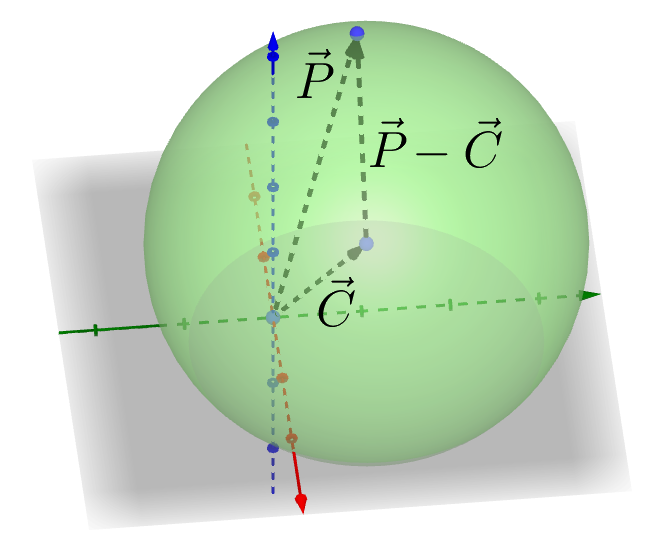
\includegraphics[scale=0.85]{sphere.png}
        \end{figure}
        
        Sea $R$ el radio de la esfera y $\vec{C}=(x_0, y_0, z_0)$ el centro. Sea $\vec{P}=(x,y,z)$ el vector de posición que va a barrer toda la esfera. Entonces requerimos que la distancia entre $\vec{P}$ y $\vec{C}$ sea siempre igual al radio $R$, es decir:
        \begin{align}
            \Abs{\vec{P} - \vec{C}} &= R \label{sphereEquation}
        \end{align}
        
        Si reemplazamos cada vector por sus componentes, entonces:
        \begin{align}
            &\Abs{(x-x_0, y-y_0, z-z_0)} = R \nonumber \\
            &\implies (x-x_0)^2 + (y-y_0)^2 + (z-z_0)^2 = R^2 \label{sphereEquation2}
        \end{align}
        
        Esta ecuación es muy parecida a la del círculo, simplemente incluimos la componente en $\mathbf{z}$.
        
        % =========================================================
        % =============     DISTANCIA PUNTO-RECTA   ===============
        % =========================================================
            
        \clearpage    
            
        \section{Distancia punto-recta}
        
            Supongamos que tenemos una línea en su forma paramétrica $\vec{r} = \lVec{a_0} + t\vec{v}$ y un punto $\vec{P}$. Queremos saber la mínima distancia que hay entre $\vec{P}$ y la línea.
        
            \subsection{Método 1}
            ¿Recuerdas la definición \ref{vectorProjection} de la proyección de un vector sobre otro? La retomaremos aquí.
            
            \begin{figure}[H]
                \centering
                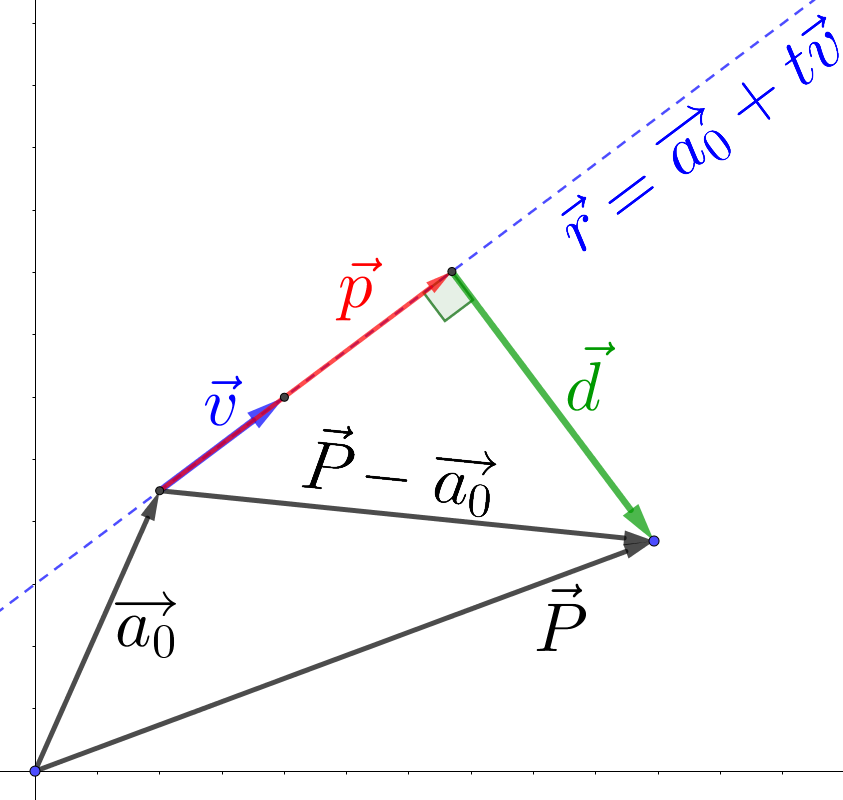
\includegraphics[scale=1.65]{distancePointLine.png}
            \end{figure}
        
            De la figura vemos que el vector $\vec{P}-\lVec{a_0}$ tiene el mismo origen que el vector paralelo a la línea, que es $\vec{v}$. Por definición de distancia punto-línea, queremos la más corta, es decir, la longitud del segmento que resulta de proyectar ortogonalmente el vector $\vec{P}-\lVec{a_0}$ sobre la línea.
            
            Y ya tenemos la fórmula para eso. Sea $\vec{d}$ el vector resultado de dicha proyección, entonces, por la ecuación \ref{defProj2}, tenemos que:
            \begin{align}
                \vec{d} &= \Wrap{\vec{P} - \lVec{a_0}} - \Wrap{\Wrap{\vec{P} - \lVec{a_0}} \dotP \hat{v}} \hat{v} \label{distancePointLine}
            \end{align}
            
            De esa forma, la distancia que queremos es justamente la magnitud de $\vec{d}$:
            \begin{align}
                &\Abs{\vec{d}} = \Abs{\Wrap{\vec{P} - \lVec{a_0}} - \Wrap{\Wrap{\vec{P} - \lVec{a_0}} \dotP \hat{v}} \hat{v}}\\
                &\Abs{\vec{d}} = \Abs{\Wrap{\vec{P} - \lVec{a_0}} - \dfrac{\Wrap{\vec{P} - \lVec{a_0}} \dotP \vec{v}}{\Abs{\vec{v}}^2} \vec{v}} \label{distancePointLine1}
            \end{align}
            
            \subsection{Método 2}
            Ahora usaremos un poco de trigonometría y el producto cruz. Retomemos la figura anterior:
            
            \begin{figure}[H]
                \centering
                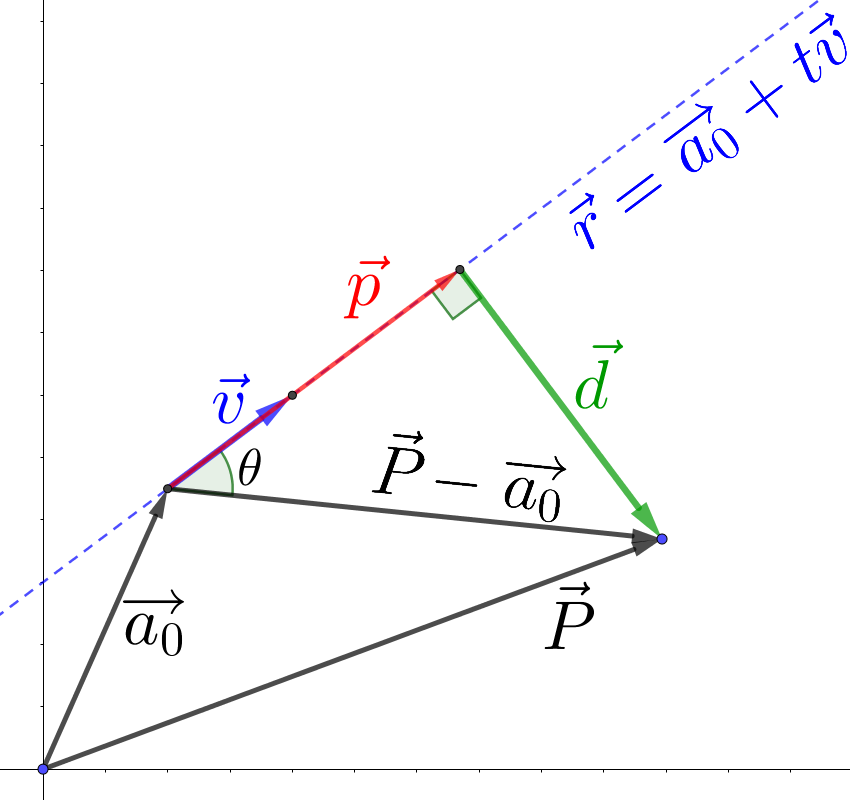
\includegraphics[scale=1.65]{distancePointLine2.png}
            \end{figure}
        
            Sea $\theta$ el ángulo que forman los vectores $\vec{v}$ y $\vec{P} - \lVec{a_0}$. Entonces, por definición del seno en el triángulo rectángulo formado tenemos que:
            \begin{align}
                \Abs{\vec{d}} = {\Abs{\vec{P} - \lVec{a_0}}} \sin \theta
            \end{align}
            
            Y por la ecuación \ref{angleBetweenVectorsCross} sabemos que:
            \begin{align}
                \sin \theta = \dfrac{\Abs{\vec{v} \times \Wrap{\vec{P} - \lVec{a_0}}}}{\Abs{\vec{v}} \Abs{\vec{P} - \lVec{a_0}}}
            \end{align}
            
            Entonces:
            \begin{align}
                \Abs{\vec{d}} = {\cancel{\Abs{\vec{P} - \lVec{a_0}}}} \dfrac{\Abs{\vec{v} \times \Wrap{\vec{P} - \lVec{a_0}}}}{\Abs{\vec{v}} \cancel{\Abs{\vec{P} - \lVec{a_0}}}} = \dfrac{\Abs{\vec{v} \times \Wrap{\vec{P} - \lVec{a_0}}}}{\Abs{\vec{v}}} \label{distancePointLine2}
            \end{align}
            
                \subsubsection{Caso particular: línea en el plano xy}
                Supongamos que tenemos una línea en el plano xy cuya ecuación es $ax+by=c$, y un punto $P$ cuyo vector de posición es $\vec{P}=(x_0, y_0)$. Para hallar la distancia entre este punto y la recta, primero tenemos que parametrizarla.
                
                Vemos que $y=-\dfrac{a}{b}x+\dfrac{c}{b}$, por lo tanto $\vec{r} = (x, y) = \Wrap{x, -\dfrac{a}{b}x+\dfrac{c}{b}} = \Wrap{0, \dfrac{c}{b}} + x\Wrap{1, -\dfrac{a}{b}}$. De esa forma $\lVec{a_0}=\Wrap{0, \dfrac{c}{b}}$ y $\vec{v}=\Wrap{1, -\dfrac{a}{b}}$.
                
                Sustituimos en la ecuación \ref{distancePointLine2} y obtenemos:
                \begin{align}
                    &\Abs{\vec{d}} = \dfrac{\Abs{\Wrap{1, -\dfrac{a}{b}} \times \Wrap{x_0, y_0 - \dfrac{c}{b}}}}{\Abs{\Wrap{1, -\dfrac{a}{b}}}} = \dfrac{\abs{y_0 - \dfrac{c}{b} + \dfrac{a}{b}x_0}}{\sqrt{1 + \Wrap{\dfrac{a}{b}}^2}} \nonumber \\
                    &\implies \Abs{\vec{d}} = \dfrac{\abs{ax_0 + by_0 - c}}{\sqrt{a^2 + b^2}} \label{distancePointLine3}
                \end{align}
            
            \clearpage
            
            \subsection{Extra: reflexión de un punto sobre una recta}
            Ahora supongamos que la línea es un espejo y queremos hallar un punto $\vec{P'}$ tal que esté del otro lado de la línea y tenga la misma distancia a la línea que el punto original $\vec{P}$.
            
            \begin{figure}[H]
                \centering
                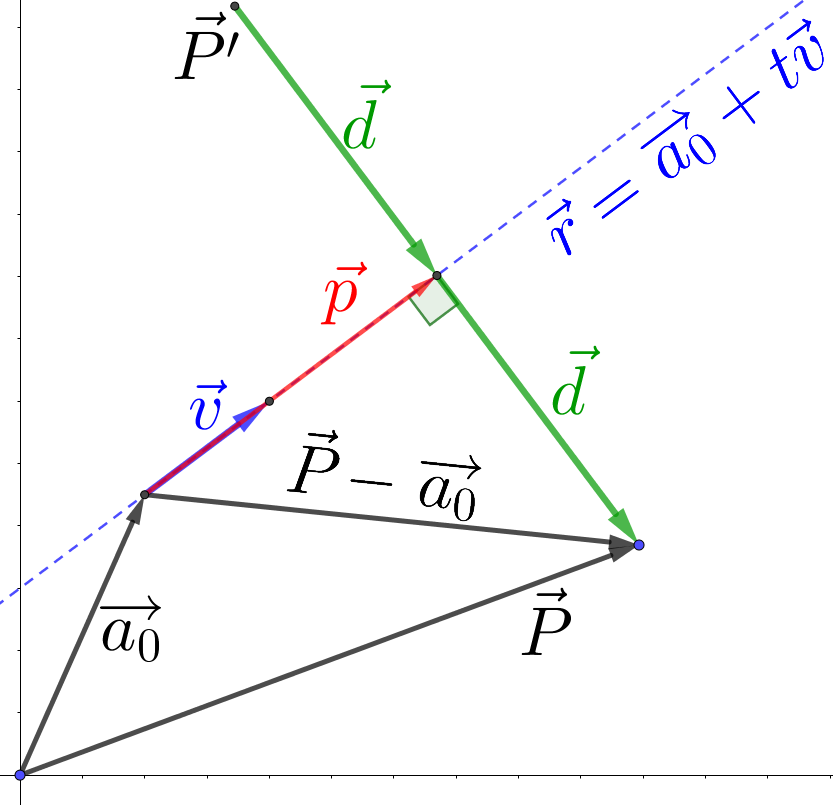
\includegraphics[scale=1.65]{reflection.png}
            \end{figure}
        
            Vemos que necesitamos otra vez el vector $\vec{d}$ que ya hemos calculado en la ecuación \ref{distancePointLine}. Y obtener $\vec{P'}$ es muy sencillo, simplemente a $\vec{P}$ le sumamos dos veces el desplazamiento que indica el vector $\vec{d}$ en dirección hacia $\vec{P'}$. Pero como $\vec{d}$ va en dirección contraria a la que queremos, le invertimos el sentido y dicha suma se convierte en una resta de dos veces el vector $\vec{d}$:
            \begin{align}
                \vec{P'} = \vec{P} - 2\vec{d}
            \end{align}
            
            Finalmente sustituimos la ecuación \ref{distancePointLine}:
            \begin{align}
                &\vec{P'} = \vec{P} - 2 \Brackets{\Wrap{\vec{P} - \lVec{a_0}} - \Wrap{\Wrap{\vec{P} - \lVec{a_0}} \dotP \hat{v}} \hat{v}} \nonumber \\
                &\implies \vec{P'} = 2\lVec{a_0} - \vec{P} + 2\Wrap{\Wrap{\vec{P} - \lVec{a_0}} \dotP \hat{v}} \hat{v} \label{reflectionPointLine}
            \end{align}
            
            Por supuesto que no te recomiendo que te memorices todas las fórmulas anteriores (yo nunca me las aprendí), sino que cuentes con las herramientas adecuadas para poder deducirlas y aplicarlas correctamente en los problemas.
            
        % =========================================================
        % =============     DISTANCIA PUNTO-PLANO   ===============
        % =========================================================
        
        \clearpage
        
        \section{Distancia punto-plano}
        Usaremos ideas similares a las anteriores. Supongamos que tenemos un plano descrito por la ecuación $\vec{n} \dotP \Wrap{\vec{r} - \lVec{a_0}}=0$, es decir, su vector normal es $\vec{n}$, pasa por el punto $\lVec{a_0}$ y su vector de posición que lo dibuja es $\vec{r}$. Queremos hallar la mínima distancia entre un punto $\vec{P}$ y el plano.
        
        \begin{figure}[H]
            \centering
            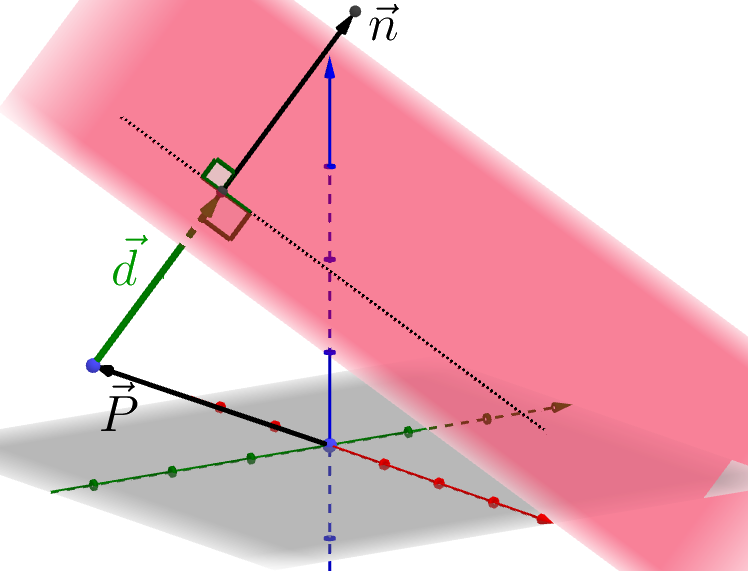
\includegraphics[scale=0.8]{distancePointPlane.png}
        \end{figure}
        
        Proyectamos ortogonalmente el punto $\vec{P}$ sobre la superficie del plano y llamemos $\vec{d}$ al vector resultante. Claramente vemos que la dirección de $\vec{d}$ es la misma que la del vector normal $\vec{n}$, entonces podemos escribir:
        \begin{align}
            \vec{d} = \Abs{\vec{d}} \hat{n}
        \end{align}
        
        Como el punto descrito por el vector de posición $\vec{P}+\vec{d}\;$ pertenece al plano, debe satisfacer la ecuación del plano. Por lo tanto, sustituimos $\vec{r}$ por $\vec{P}+\vec{d}$:
        \begin{align}
            \vec{n} \dotP \Wrap{\vec{P}+\vec{d} - \lVec{a_0}} &= 0 \nonumber \\
            \hat{n} \dotP \Wrap{\vec{P}+\Abs{\vec{d}} \hat{n} - \lVec{a_0}} &= 0 &&\Remember{Dividimos entre $\Abs{\vec{n}}$ y sustituímos $\vec{d}$} \nonumber \\
            \hat{n} \dotP \Wrap{\vec{P} - \lVec{a_0}} + \Abs{\vec{d}} &= 0 &&\Remember{Expandimos el producto punto} \nonumber \\
            \Abs{\vec{d}} &= -\hat{n} \dotP \Wrap{\vec{P} - \lVec{a_0}} &&\Remember{Despejamos} \nonumber \\
            \Abs{\vec{d}} &= \abs{\hat{n} \dotP \Wrap{\vec{P} - \lVec{a_0}}} &&\Remember{Sacamos valor absoluto por si el producto punto es negativo} \nonumber \\
            \Abs{\vec{d}} &= \dfrac{\abs{\vec{n} \dotP \Wrap{\vec{P} - \lVec{a_0}}}}{\Abs{\vec{n}}} &&\Remember{Recuerda que $\hat{n}=\dfrac{\vec{n}}{\Abs{\vec{n}}}$} \label{distancePointPlane}
        \end{align}
        
        Observa que la ecuación anterior no es más que la longitud de la proyección del vector $\vec{P} - \lVec{a_0}$ sobre el vector normal $\vec{n}$. ¿Podrías explicar por qué?
        
            \subsubsection{Caso particular: fórmula en forma cartesiana}
            
            Si descomponemos los vectores en coordenadas, es decir, $\vec{n}=(a,b,c)$, $\vec{P}=(x_1, y_1, z_1)$ y $\lVec{a_0}=(x_0, y_0, z_0)$, entonces obtenemos la fórmula en forma cartesiana:
            \begin{align}
                &\Abs{\vec{d}} = \dfrac{\abs{a(x_1 - x_0) + b(y_1 - y_0) + c(z_1 - z_0)}}{\sqrt{a^2+b^2+c^2}} \nonumber \\
                &\Abs{\vec{d}} = \dfrac{\abs{ax_1 + by_1 + cz_1 - (ax_0 + by_0 + cz_0)}}{\sqrt{a^2+b^2+c^2}} \nonumber \\
                &\Abs{\vec{d}} = \dfrac{\abs{ax_1 + by_1 + cz_1 - d}}{\sqrt{a^2+b^2+c^2}}
            \end{align}
            Donde recuerda que la ecuación del plano en forma cartesiana es $ax+by+cz=d$ (no confundas las d's).
            
        \clearpage
        
        % =========================================================
        % ============     ROTACIONES EN EL ESPACIO   =============
        % =========================================================
        
        \section{Rotaciones en el espacio}
        
        Este es una aplicación muy interesante y padre a la vez. Supongamos que tenemos una línea en el espacio y un punto, nuestro objetivo será rotarlo usando a la línea como eje mediante un ángulo determinado.
        
        
        
        % =========================================================
        % ============    DEMOSTRACIONES GEOMETRICAS   ============
        % =========================================================
        
        \section{Demostraciones geométricas mediante vectores}
        
        Muchas demostraciones en geometría se pueden simplificar y llevar a cabo usando vectores de forma más elegante. Algunas propiedades que podemos aprovechar son:
        \begin{itemize}\setlength\itemsep{0em}
            \item Expresar cada segmento de la figura con vectores de desplazamiento de una forma conveniente.
            \item También podemos expresar los vértices como vectores de posición.
            \item Para probar que dos segmentos son paralelos, probamos que los vectores que los representan tienen la misma dirección, o equivalentemente, que uno es múltiplo escalar del otro.
            \item Para probar que dos segmentos tienen la misma longitud, probamos que los vectores que los representan tienen la misma magnitud.
            \item En algunos casos podemos escoger algunos vectores como base y expresar a otros como combinación lineal de los primeros.
            \item Para hallar razones entre longitudes de segmentos, podemos usar ideas de dependencia e independencia lineal.
            \item En la mayoría de los casos no es necesario descomponer los vectores en sus componentes.
            \item El producto punto puede servir para probar perperndicularidad y en algunos casos simplificar expresiones que involucren magnitudes.
        \end{itemize}
    
        Así que, veamos muchos ejemplos:


\part{Cálculo diferencial vectorial}

    \chapter{Funciones de varias variables}
    
        \section{Representación como superficies}
        
            \subsection{Curvas de nivel y de contorno}
            
        \section{Límites}
            
            \subsection{Definición intuitiva}
            
            \subsection{Definición formal}
            
        \section{Continuidad}
        
        \section{Derivadas parciales}
        
            \subsection{Plano tangente a una superficie}
            
            \subsection{Diferenciabilidad}
            
            \subsection{Derivadas de orden superior}
            
                \subsubsection{Teorema de Clairaut}
                
        \section{Gradiente}
                
        \section{Regla de la cadena}
        
            \subsection{Diferencial total}
            
        \section{Derivada direccional}
        
        \section{Puntos críticos}
        
            \subsection{Máximos, mínimos y puntos silla}
            
            \subsection{Criterio del hessiano}
            
        \section{Multiplicadores de Lagrange}


    \chapter{Funciones vectoriales}
    
        \section{Curvas en forma paramétrica}
        
            \subsection{Reglas de derivación}
            
            \subsection{Velocidad y aceleración}
        
            \subsection{Longitud de arco}
            
            \subsection{Parametrización por longitud de arco}
            
            \subsection{Geometría diferencial}
                
                \subsubsection{Vector tangente, normal y binormal}
                
                \subsubsection{Curvatura y torsión}
                
                \subsubsection{Velocidad y aceleración}
                
                \subsubsection{Ecuaciones de Frenet-Serret}
            
        \section{Campos vectoriales}
        
            \subsection{Líneas de campo}
            
            \subsection{Derivadas parciales}
        
        \section{Operador nabla}
        
            \subsection{Gradiente}
            
            \subsection{Divergencia}
            
            \subsection{Rotacional}
            
            \subsection{Laplaciano}
            
            \subsection{Propiedades}



\part{Cálculo integral vectorial}

    \chapter{Integrales multivariable}
    
        \section{Regiones}
        
            \subsection{Regiones del plano y tipos}
            
            \subsection{Regiones del espacio y tipos}
        
        \section{Integrales iteradas}
        
        \section{Integrales dobles}
            
            \subsection{Integración sobre regiones arbitrarias}
            
            \subsection{¿Cómo hallar los límites de integración?}
            
            \subsection{Teorema de Fubini}
        
        \section{Integrales triples}
            
            \subsection{Integración sobre regiones arbitrarias}
            
            \subsection{¿Cómo hallar los límites de integración?}
            
        \section{Cambio de variable en 2 y 3 dimensiones}
        
            \subsection{Transformación de coordenadas}
            
            \subsection{Jacobiano}
            
        \section{Aplicaciones}
        
            \subsection{Valor promedio}
            
            \subsection{Centro de masa}
            
            \subsection{Momento de inercia}
        
    \chapter{Integrales de funciones vectoriales}
    
        \section{Integrales de línea}
        
            \subsection{Función escalar}
            
            \subsection{Función vectorial}
            
            \subsection{Campos conservativos}
            
                \subsubsection{Potencial}
        
        \section{Integrales de superficie}
        
            \subsection{Superficies en forma paramétrica}
            
                \subsubsection{Vector normal}
            
                \subsubsection{Relación con el Jacobiano}
                
                \subsubsection{Cálculo a través del gradiente}
            
            \subsection{Función escalar}
            
            \subsection{Función vectorial}
        
        \section{Integrales de volumen}
        
            \subsection{Regiones del espacio en forma paramétrica}
            
                \subsubsection{Elemento de volumen}
                
                \subsubsection{Relación con el Jacobiano}
        
            \subsection{Función escalar}
            
        \section{Consejos para parametrizar y definir límites}
    
    \chapter{Teoremas de integración}
    
        \section{Teorema de Green}
        
            \subsection{Cálculo de áreas dado el contorno}
        
        \section{Teorema de Stokes}
        
            \subsection{Frontera de una superficie}
        
        \section{Teorema de la divergencia de Gauss}
        
            \subsection{Superficie cerrada}


\part{Coordenadas curvilíneas}

    \chapter{Coordenadas curvilíneas generalizadas}
    
        \section{Transformación de coordenadas}
        
        \section{Sistemas ortogonales}
        
        \section{Vectores unitarios}
        
            \subsection{Factores de escala}
        
        \section{Integración}
        
            \subsection{Elemento de línea}
            
            \subsection{Elemento de longitud de arco}
            
            \subsection{Elemento de área}
            
            \subsection{Elemento de volumen}
            
        \section{Operador nabla}
        
            \subsection{Gradiente}
            
            \subsection{Divergencia}
            
            \subsection{Rotacional}
            
            \subsection{Laplaciano}
            
        \section{Sistemas comunes de coordenadas}
        
            \subsection{Cilíndricas}
            
            \subsection{Esféricas}
            

\end{document}
